\documentclass[12pt,onecolumn,a4paper]{book}
\usepackage{epsfig,amsthm,amsmath,booktabs,csquotes}
\usepackage [pagebackref=true, colorlinks, linkcolor=blue, citecolor=magenta, urlcolor=cyan] {hyperref}
\usepackage{color,xcolor}

\usepackage{titlesec} %include more subsection than subsubsection

\usepackage{pdflscape}
\usepackage{geometry}
\usepackage{dialogue,attrib,lips}

\usepackage{caption}
\usepackage{subcaption}

\usepackage[labelformat=parens,labelsep=quad, skip=3pt]{caption}
\usepackage{graphicx}
\usepackage{enumerate,braket,tcolorbox}
\usepackage[localise]{xepersian}
%\settextfont[Scale=1.2]{‌BNAZANIN.TTF}
%\settextfont[Scale=1.2]{BZAR.TTF}
\settextfont[Scale=1]{XB Niloofar}
\ExplSyntaxOn
\cs_set_eq:NN
\etex_iffontchar:D
\tex_iffontchar:D
\cs_undefine:N \c_one
\int_const:Nn \c_one { 1 }
\ExplSyntaxOff
\setdigitfont[Scale=1]{XB Niloofar}
\setlatintextfont[Scale=1]{Times New Roman}

% set local changes to margin
\def\changemargin#1#2{\list{}{\rightmargin#2\leftmargin#1}\item[]}
\let\endchangemargin=\endlist 
%

% newcommands
\newcommand{\floor}[1]{\left\lfloor #1 \right\rfloor}
\newcommand{\ceil}[1]{\left\lceil #1 \right\rceil}
% -------------------- Enviroments --------------------
\newenvironment{mohsenletter}
{
	\begin{tcolorbox}[title = صندوق پیام‌ها]
		\begin{dialogue}
		}
		{
		\end{dialogue}
	\end{tcolorbox}
}

\newenvironment{meeting}
{
	\begin{tcolorbox}[title = دیدار]
		\begin{dialogue}
		}
		{
		\end{dialogue}
	\end{tcolorbox}
}


% -------------------- Document --------------------

\begin{document}
\title{مطالعه همگامی در شبکه‌های عصبی مهاری} 
\author{محسن مهرانی - استاد راهنما: دکتر سامان مقیمی عراقی}
\date{}
\maketitle
\tableofcontents
\newpage
\فصل{سخن نخست}
مطالعه فعالیت شبکه‌های عصبی برای تحقیق و بررسی کارکردهای مغز اهمیت زیادی دارد. همه بر این باوریم که مغز محمل اندیشه و تفکر است. ما کنجکاو هستیم که چگونه همکاری بین نورون‌های آن باعث می‌شود تا حافظه، کشف و پردازش صورت گیرد. هر کدام از نورون‌های مغز می‌تواند در حالت فعال [روشن] یا غیرفعال [خاموش] قرار گیرد. هم اکنون شواهدی وجود دارد که علائم بیماری عصبی «صرع» در زمان‌هایی رخ می‌دهند که الگوی خاموش و روشن شدن نورون‌های مغز باهم \textbf{«هم‌گامی»} دارند. هم‌گامی به این معناست که جمعیت بزرگی از نورون‌ها باهم خاموش و روشن می‌شوند و یک الگوی تکرار شونده‌ای را دنبال می‌کنند. تو گویی که باهم هم‌آهنگ یا هم‌گام شده‌اند.\\

بی‌تردید دستیابی به تمام جزییات مغز برای ما میسّر نیست و به آن به عنوان یک \textbf{«جعبه‌ی سیاه»} نگاه می‌کنیم که مدت‌هاست به دنبال ارائه مدلی هستیم که رابطه‌ی بین ورودی‌ها و خروجی‌های ثبت شده را بازتولید کند. کاری که در این پژوهش انجام خواهیم داد تلاشی است برای پیشنهاد دادن یک مدل برای این جعبه‌ی سیاه که رفتار نسبتا مشابهی را میان ورودی و خروجی‌های این جعبه سیاه شبیه‌سازی می‌کند. همچنین به کمک بررسی دقیق‌تر این مدل تلاش می‌کنیم تا نقطه‌ی تقریبی گذرفاز سامانه را از فاز ناهم‌گام به هم‌گام پیدا کنیم.

\قسمت{مقدمه}
مدل‌های زیادی برای شبکه‌های عصبی ارائه شده است که توانایی تولید رفتار هم‌گام شدن نورون‌ها را در آن‌ها می‌توانیم جستجو کنیم. یکی از این مدل‌ها که در تمام فصول شبیه‌سازی از آغاز تا کنون از آن بهره برده شده است؛ مدل انباشت و شلیک است\cite{PhysRevLett.105.158104}. در این جستار ابتدا با مدل انباشت و شلیک شروع می‌کنیم و سپس به مدلی توسعه یافته که آن را \textbf{«چرخنده»} صدا خواهیم کرد؛ می‌پردازیم.\\

متن اصلی این جستار شامل معرفی این مدل‌ها و پویایی آن‌ها در زمان و نتایج ضبط شده از آشکارسازهایی است که وجود هم‌گامی را شکار می‌کنند.

\فصل{شبکه انباشت و شلیک}
در این نوشتار \cite{PhysRevLett.105.158104}  نویسندگان تلاش می‌کنند تا هم‌گامی را برای شبکه‌ی نورون‌های مهاری رصد کنند. این نورون‌ها به گونه‌ای باهم مرتبط هستند که تیزه زدن هر نورون منجر به مهار پتانسیل دیگر نورون‌ها می‌شود. تک‌تک نورون‌های این شبکه از تحول انباشت و شلیک تبعیت می‌کند. معادله تحول اختلاف پتانسیل هر کدام از نورون‌ها با محیط بیرونش از رابطه زیر داده می‌شود:
\begin{tcolorbox}
	\begin{align}
		\dot{v_i}=a_i - v_i - \frac{g}{N} \sum_{n|t_n<t} S_{i,l(n)} \delta(t - t_n - t_d) 
		\label{eq:potential_1}
	\end{align}
	
	\begin{enumerate}[-]
		\item
		$g$: 
		ضریب اتصال هر جفت نورون. از آن‌جا که همه‌ی نورون‌ها در این مطالعه مهاری هستند؛ باید این کمیت مثبت انتخاب شود تا تاثیر جمله‌ی پایانی در نهایت منفی باشد.
		\item
		$S$:
		ماتریس همسایگی. این کمیت نشان می‌دهد که آیا دو نورون به هم متصل و تاثیرگذار هستند یا خیر.
		\item
		$t_d$: 
		زمان تاخیر میان زدن تیزه هر نورون و تاثیر آن روی نورون‌های دیگر.
		\item
		$a_i$:
		یک پتانسیل تحریکی و خارجی. در این مطالعه این مقدار برای هر نورون به صورت تصادفی انتخاب می‌شود و تا پایان شبیه‌سازی ثابت باقی می‌ماند.
		\item
		$N$:
		تعداد نورون‌های در شبکه
	\end{enumerate}
\end{tcolorbox}
\زیرقسمت{آهنگ تیزه زدن}
پیش از آن که به شبیه‌سازی یک شبکه‌ از نورون‌ها بپردازیم؛ خوب است تا یک نورون تنها را مطالعه کنیم. یک نورون تنها که پویایی از جنس مدل انباشت‌وشلیک دارد؛ دوره تناوب تیزه‌زدن آن از رابطه‌ی زیر قابل محاسبه است .
\begin{align}
	\dot{v_i}= I  - v_i &\rightarrow \frac{dv_i}{I - v_i} = dt \\
	&\rightarrow T = ln(\frac{I}{I - 1})
\end{align}
این رابطه نشان می‌دهد که بسامد تیزه‌زدن یک نورون با افزایش مجموع جریان‌های ورودی آن به صورت لگاریتمی افزایش می‌یابد.
\زیرقسمت{نشانگر تشخیص فاز هم‌گامی}
برای آن که متوجه شویم که شبکه در حالت هم‌گامی یا ناهم‌گامی است نیاز است تا آشکارسازی را تعبیه کنیم که باتوجه به رفتار سامانه، هم‌گامی یا ناهم‌گامی را با عقربه‌ی خود نشان دهد. برای این منظور ابتدا مفهوم میدان ($E$) را تعریف می‌کنیم که بیانگر شدت فعالیت نورون‌های شبکه است. انحراف از معیار این کمیت در طول زمان، پارامتر مناسبی است که به کمک آن هم‌گامی را تشخیص دهیم.
\begin{tcolorbox}
	\begin{align}
		\ddot{E}+ 2\alpha \dot{E}+\alpha^{2}E &=\frac{\alpha^2}{N} \sum_{n|tـn<t} \delta(t - t_n - t_d) \\
		\sigma^{2} &= \braket{E^{2}}_{t} - \braket{E}^{2}_{t}
	\end{align}
	*دقت کنیم که شدت میدان با تعداد تیزه زدن‌ها رفتاری ملایم دارد. به عنوان مثال اگر تیزه‌ها متوقف شوند؛ شدت میدان پس از لحظاتی چند [متناسب با $\alpha$] صفر می‌شود.
\end{tcolorbox}

در طول زمان میدان $E$ و $\sigma$ را رصد می‌کنیم. برای دریافت شهودی عملکرد مناسب این پارامتر نظم، فرض کنید که شبکه در حالتی است که جمعیت بزرگی از آن در حال خاموش و روشن شدن هم‌گام است. پس مشاهده خواهم کرد که میدان که شدت فعالیت نورون‌ها را نشان می‌دهد در حال ضربان رفت و برگشتی است. این افت‌وخیز با تقویت هم‌گامی دامنه‌ی بزرگتر پیدا می‌کند به طوری که انحراف آن از میانگین پهنای قابل توجهی کسب می‌کند. از این رو انحراف معیار میدان، کمیت مناسبی است که میزان هم‌گامی را گزارش کند.\\

\subsection{مسائل پیشروی پیاده سازی شبیه سازی}
\subsubsection{تابع بی‌کران دلتا}
یکی از مشکلات شبیه سازی معادلات دیفرانسیلی حضور تابع دلتای دیراک است. این تابع در نقطه صفر خود دارای مقداری بینهایت است. معرفی چنین تابعی به رایانه کاری دشوار است و همانندی محاساتی ندارد. حال برای برطرف کردن این مشکل چه باید کرد؟ نکته در این جا نهفته است که چون ما برای حل عددی معادله دیفرانسیلی خود از زمان پیوسته استفاده نمی‌کنیم و از گام‌هایی با طول مثبت $\Delta t$ استفاده می‌کنیم این مشکل به صورت زیر مدیریت می‌شود.
\begin{align}
	v_{i}(t+\Delta t) &= v_{i}(t) + \int_{t}^{t+\Delta t} \dot{v_i}  dt \\
	&= v_{i}(t) + \int_{t}^{t+\Delta t} \left[ a_i - v_i - \frac{g}{N} \sum_{n|t_n<t} S_{i,l(n)} \delta(t - t_n - t_d)  \right]   dt \\
	&\approx v_{i}(t) +  \left[ a_i - v_i(t) \right] \Delta t - \frac{g}{N} \sum_{n|t_n<t} S_{i,l(n)} \int_{t}^{t+\Delta t} \delta(t - t_n - t_d) dt  \\
	&\approx v_{i}(t) +  \left[ a_i - v_i(t) \right] \Delta t - \frac{g}{N} \sum_{n|t_n<t} S_{i,l(n)} H(t + \Delta t- t_n - t_d) \label{eq:potential_changes}
\end{align}

حالا تابع پله کاملا برای ما آشنا و قابل مدلسازی است. دقت شود که تابع پله یاد شده فقط در محدوده $t, t+\Delta t$ زندگی می‌کند و پس از آن اعتبار ندارد. معادله \ref{eq:potential_changes}  می‌گوید که باید برای تحول پتانسیل نورون $i$ام بررسی کنیم که آیا نورونی در همسایگی آن تیزه زده است یا نه. اگر چنان باشد؛ یک واحد به جمع تیزه زدگان اضافه کنیم.


\subsubsection{ثبت تاریخ تیزه زدن‌ها}
برای محاسبه تحول پتانسیل در رابطه \ref{eq:potential_changes} چنان که توضیح داده شد نیاز به دانستن تاریخ تیزه زدن‌ها داریم. اگر بخواهیم برای تمامی نورون‌ها در هر گام زمانی تیزه‌زدن آن را به صورت مجزا ثبت کنیم؛یک آرایه مربعی خواهیم داشت که شماره سطر آن می‌تواند معرف زمان باشد و ستون نماد شماره نورون - شکل شماره (\ref{fig:rasterplot}).\\

اما مشکلی که برای این شبیه سازی رخ خواهد داد. در صورت افزایش تعداد نورون‌ها و زمان شبیه سازی با یک ابر آرایه روبرو خواهیم شد که امکان دارد در ذخیره سازی آن دچار مشکل شویم. به همین خاطر در شبیه سازی انجام شده تنها مجموع تیزه زدن‌ها را ذخیره کردیم تا یک آرایه یک ستونه داشته باشیم و در ذخیره‌سازی به مشکل نخوریم.

\subsection{نتایج}
اندازه‌ی پارامتر‌هایی که برای این شبیه‌سازی انتخاب کردیم؛ کاملا از صورت مقاله یاد شده برداشته شده و به قرار زیر است.
\begin{tcolorbox}[colback=green!5!white,colframe=green!75!black]
	\begin{enumerate}[*]
		\item
		$\alpha = 20\, s^{-1}$
		\item
		جریان‌های تصادفی خارجی نورون‌ها از اعضای بازه‌ی $(1.2,2.8)$ انتخاب می‌شوند.
		\item
		$N = 10000$
		\item
		$t_d = 0.1\, s$ 
	\end{enumerate}
\end{tcolorbox}
این شبیه سازی برای ۱۰۰۰ ثانیه اجرا شده است که در آن هر گام زمانی برابر $0.01$ ثانیه گرفته شده است. کد شبیه‌سازی در پوشه 
\href{run://..//scripts//kuramoto_model_synchoronization_problem}{مسئله همگامی برای مدل انباشت‌و‌شلیک}
قابل مشاهده است.
\begin{figure}
	\begin{subfigure}[b]{0.5\textwidth}
		\centering
		\includegraphics[width = \textwidth]{../scripts/kuramoto_model_synchoronization_problem/single_runs/N1000_T1000_g5_input_1.2_2.8/raster_plot.png}
		\caption{ثبت لحظه‌ای تیزه زدن هر نورون به صورت مجزا - در این نمودار ضریب تاثیر هر نورون روی همسایه‌هایش $g = 5$ بوده است. چنان که انتظار می‌رفت شاهد هم‌گامی هستیم.}
		\label{fig:rasterplot}
	\end{subfigure}
	\hfill
	\begin{subfigure}[b]{0.5\textwidth}
		\centering
		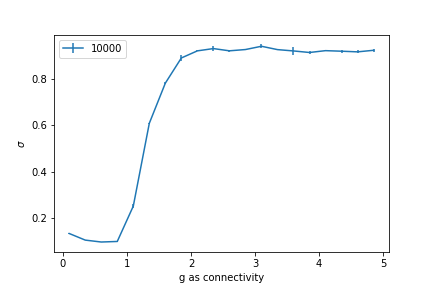
\includegraphics[width =  \textwidth]{../papers_studies/figs/IF/sigma.png}
		\caption{تغییر فاز از ناهم‌گامی به هم‌گامی برای ۱۰۰۰ نورون}
		\label{fig:if_phase_transition}
	\end{subfigure}
	\hfill
	\begin{subfigure}[b]{0.5\textwidth}
		\centering
		\includegraphics[width = \textwidth]{../scripts/all_neurons_model_in_one_place/IF_ensembles/N10000_T1000_I1.2_2.8_cluster_computed/silent_neurons_g_0.1_65.png}
		\caption{آمار نورون‌های خاموش درون سامانه}
		\label{fig:if_silent_neurons}
	\end{subfigure}
	\hfill
	\begin{subfigure}[b]{0.5\textwidth}
		\centering
		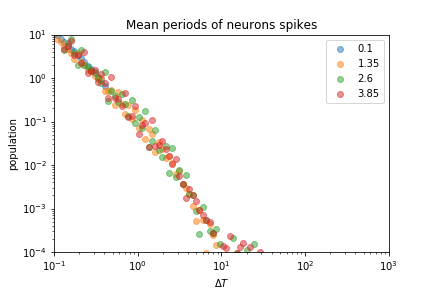
\includegraphics[width = \textwidth]{../papers_studies/figs/IF/mean_spiking_persiods.png}
		\caption{توزیع بسامدی شبکه‌های ۱۰۰۰ نورونی که هر کدام قدرت اتصال متفاوتی دارند. }
		\label{fig:if_isi}
	\end{subfigure}
	\hfill
	\begin{subfigure}[b]{0.5\textwidth}
		\centering
		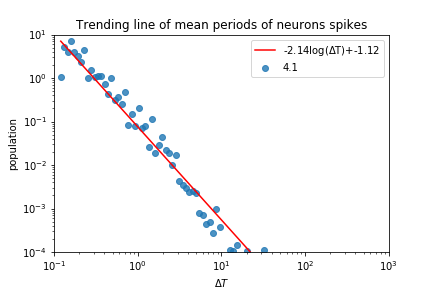
\includegraphics[width = \textwidth]{../papers_studies/figs/IF/mean_spiking_persiods_with_trending_line.png}
		\caption{محاسبه‌ی نمای توزیع توانی فاصله زمانی بین تیزه‌ها}
		\label{fig:if_isi_trending_line}
	\end{subfigure}
	\hfill
	\begin{subfigure}[b]{0.5\textwidth}
		\centering
		\includegraphics[width = \textwidth]{../scripts/all_neurons_model_in_one_place/IF_ensembles/N10000_T1000_I1.2_2.8_cluster_computed/sigma_phase_space_contour.png}
		\caption{صفحه‌ی فاز مربوط به سامانه‌ی نورون‌های انباشت‌وشلیک: پیوست \ref{appendix:phase_sampling_if}}
		\label{fig:if_g_d_phase_space_if}
	\end{subfigure}
\end{figure}

\زیرزیرقسمت{انحراف از معیار میدان}
مهم‌ترین شاخصه ما برای ردگیری همگامی، انحراف معیار میدان $E$ است که با زیگما $\sigma$ نمایش می‌دهیم. جهش به وجود آمده در شکل‌ (\ref{fig:if_phase_transition}) به این معنی است که سامانه از حالت ناهم‌گامی به هم‌گامی تغییر فاز داده است. 



\زیرزیرقسمت{نورون‌های خاموش}
بی‌تردید میدان داخلی نورون‌ها کاملا تابعی است از آمارتیزه‌های درون سامانه. نورون‌هایی که گاهی برای تیزه زدن به پیش می‌روند و گاه به علت حضور میدان داخلی مهار به عقب برمی‌گردند. خوب است بپرسیم که برآیند این رفت و برگشت‌ برای هر نورون چگونه است. آیا این رفت و برگشت منجر به رسیدن به آستانه‌ی تیزه زدن می‌شود و یا نورون در برآیند اصلا پیشروی نمی‌کند و هیچگاه به آستانه نمی‌رسد و خاموش می‌ماند.\\
در شکل \ref{fig:if_silent_neurons} شمار نورون‌هایی که هیچگاه در سامانه تیزه نمی‌زنند را آورده‌ایم و این که چگونه با با افزایش ضریب تاثیر مهاری میدان این آمار رشد می‌کند.\\
این مشاهده نشان می‌دهد که در فاز هم‌گام، تقریبا ۲۵ درصد نورون‌ها خاموش هستند و نقشی در برقراری جریان داخلی ندارند. قابل حدس است که نورون‌هایی خاموش هستند که جریان‌های تصادفی خارجی پایین دست را داشته‌اند. به این معنی که اگر بازه‌ی جریان تصادفی را تنگ‌تر می‌گرفتیم [ مثلا از$1.6$ ] شروع می‌کردیم؛ سامانه در فاز هم‌گام تفاوت رفتاری نمی‌داشت.\\
همچنین جالب است که تغییر فاز مشاهده شده در تعداد نورون‌های خاموش - شکل \ref{fig:if_silent_neurons}-در حالتی در همسایگی و متمایز از تغییر فاز شکل \ref{fig:if_phase_transition} نشان می‌دهد.


\زیرزیرقسمت{توزیع تناوب زمانی تیزه‌ها}
شبکه‌ی ما متشکل از نورون‌هایی است که مدام در حال تیزه زدن و فعال نگه‌داشتن شبکه هستند. برخی با بسامد بیشتری تیزه می‌زنند و برخی آهسته‌تر. اگر کنجکاو باشیم که جمعیت کل نورون‌های ما چگونه میان دسته‌های مختلف با تناوب‌های متفاوت توزیع شده‌ است؛ لازم است تا توزیع فراوانی آن‌ها را یکجا رسم کنیم - شکل \ref{fig:if_isi}.\\
همان طور که می‌بینید به ظاهر این توزیع رفتاری توانی دارد و اگر کنجکاو باشیم می‌توانیم شیب این نمودار تمام لگاریتمی آن را جهت محاسبه‌ی نمای توزیع بدست آوریم - شکل \ref{fig:if_isi_trending_line}.

\زیرقسمت{پهن‌کردن قالی صفحه‌ی فاز}
در قسمت‌های پیشین تنها به مطالعه‌ی تاثیر ضریب اتصال در تغییرفاز پرداختیم و زمان تاخیر را تنها در $t_d = 0.1 s$ خلاصه کردیم. حال اجازه دهید تا به تاخیر نیز اجازه‌ی تغییر دهیم. در ادامه‌ی این قسمت از نوشتارمان، به فرش‌کردن صفحه‌ی فاز خود خواهیم پرداخت. امید است که چهره‌ی تمام نمای سامانه‌ بر صورت این قالی نقش بندد.\\


\زیرزیرقسمت{قالی انحراف از معیار میدان}
در شکل \ref{fig:if_g_d_phase_space} مشاهده می‌کنیم که شدت هم‌گامی در هر کدام از هنگردهای سامانه چقدر است. بنظر می‌رسد که با افزایش زمان تاخیر و ضریب تاثیر همگامی قدرت پیدا می‌کند و هر دو در ظهور این رفتار شریک هستند. اگر چه تاخیر در جابجایی ضریب‌تاثیر بحرانی تغییری ایجاد نکرده است اما هم‌گامی را قدرت می‌بخشد.


%\فصل{تصویرسازی سامانه‌ها}
	\label{chap:animations}
در فصل‌های گذشته تنها با ثبت عددی خروجی‌های مدلسازی سروکار داشتیم. خروجی‌ها تلاش داشتند تا رفتار سامانه را به ما بشناسانند. ما نیز تلاش کردیم تا بررسی اشکال و نمودارها آنچه را که در پس‌پرده [جعبه سیاه] می‌گذرد؛ «حدس» بزنیم. به همین دلیل برآن شدیم تا روشی برای به تصویر کشیدن سامانه ابداع کنیم تا از لحظه‌لحظه‌ی سامانه با خبر شویم، شکل \ref{fig:if_animation_plot}.
.
\begin{figure}[!h]
	\centering
	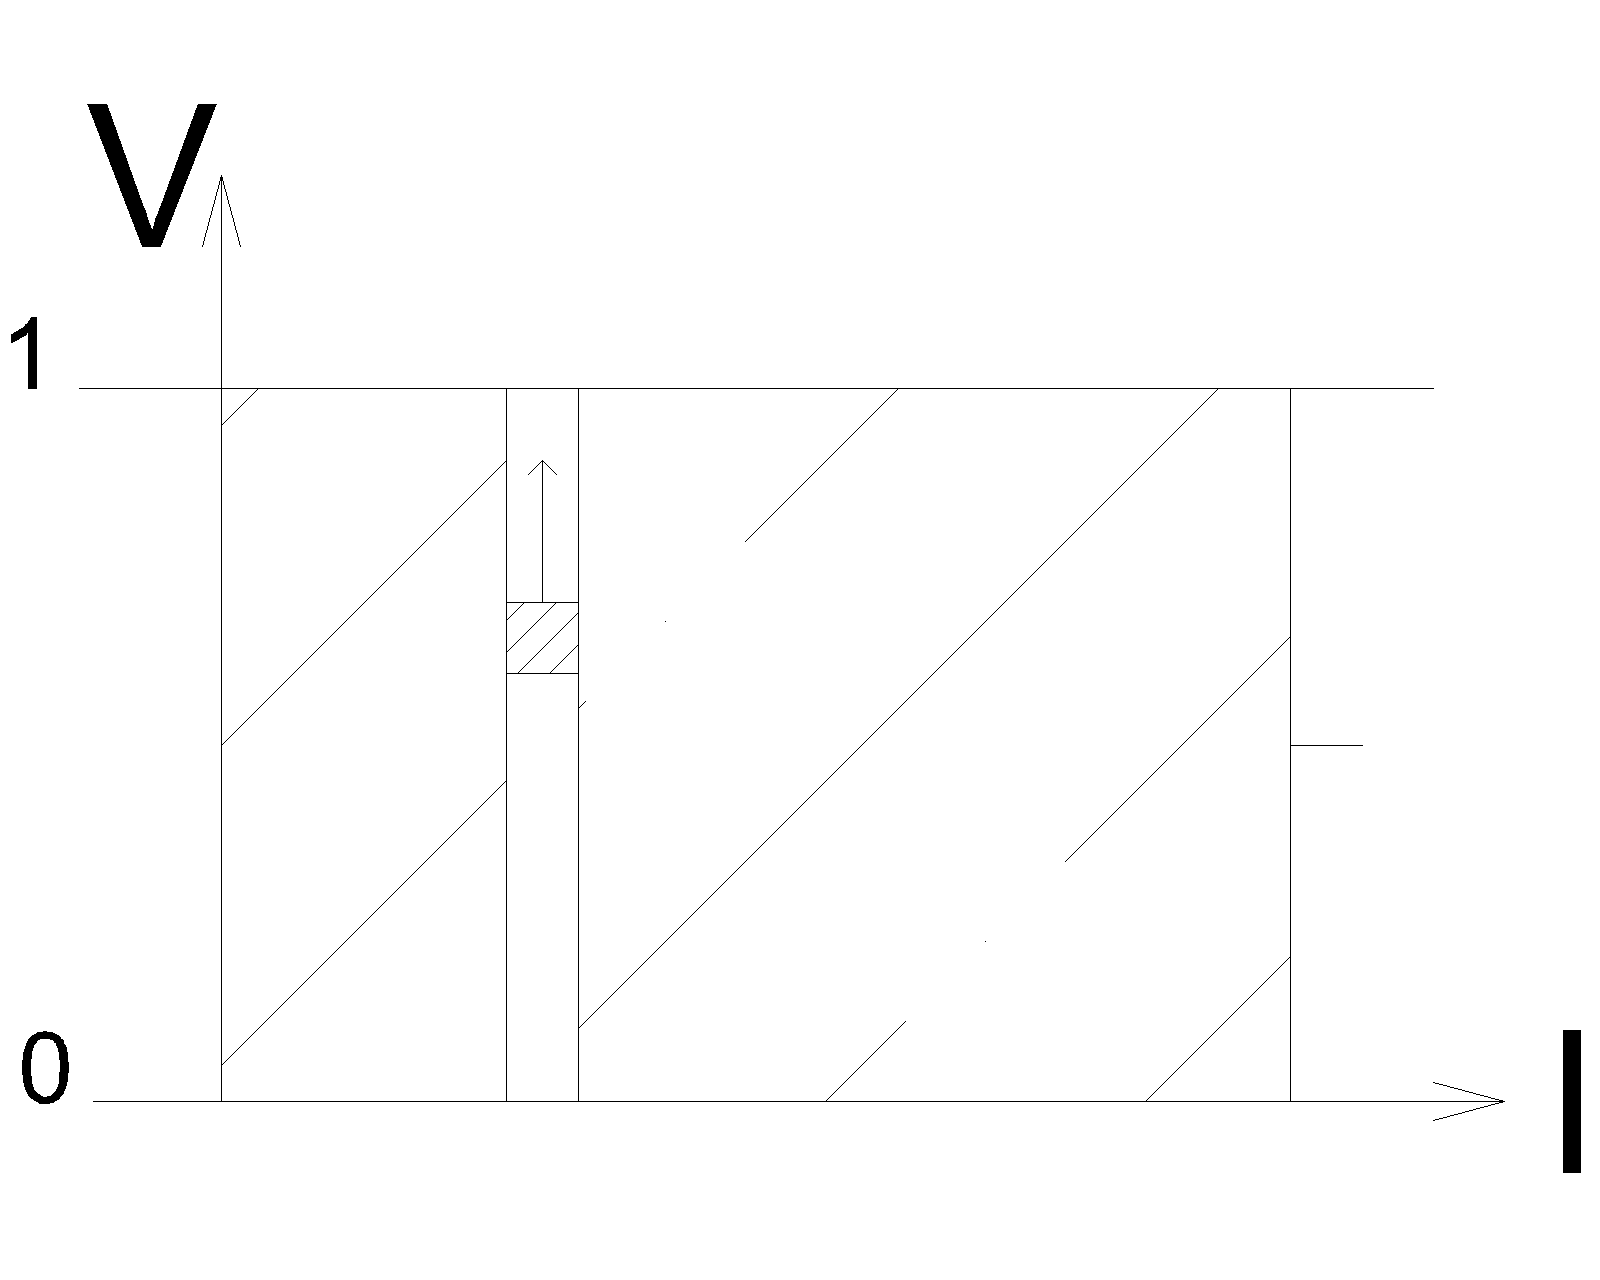
\includegraphics[width =0.8\textwidth]{../papers_studies/figs/IF/IF_phase_space-Model.png}
	\caption{تصویر فضای فاز سامانه نورونی انباشت‌وشلیک.}
	\label{fig:if_animation_plot}
\end{figure}

هر نقطه در این صفحه نمایانگر حالت یک نورون است. محور افقی نشان دهنده‌ی جریان ثابت خارجی است که به هر نورون در ابتدا متصل کرده‌ایم و محور عمودی نشان دهنده‌ی پتانسیل نورون است. پویایی شکل \ref{fig:if_animation_plot} به ما نشان خواهد داد که چگونه سامانه در زمان متحول می‌شود. طبق توصیفی که از پویایی سامانه‌ی خود داریم؛ توقع داریم که نورون‌هایی که از آستانه عبور کردند؛ مجددا از محور صفر پیدا شوند. در این قسمت، مکاتبه‌ای با استاد داشتم که می‌توانید برای مطالعه‌ی آن به پیوست 
\ref{appendix:letter_14001222}
مراجعه کنید.\\
حال بیایید تا پویایی مدل‌های مختلف سامانه‌های نورونی را از این طریق رصد کنیم. به این ترتیب که برای هر کدام از نقاطی خاص از فضای فاز مربوط به آن‌ها انتخاب می‌کنیم و می‌پرسیم که سامانه چه تصویری دارد. در شکل‌ 
\ref{fig:abc_points_neuron_models}
از هر صفحه‌ی فاز ۴ نقطه به اختصار انتخاب شده است. برای مشاهده‌ی کامل پویانمایی‌هاپوشه‌ی مربوط به هر مدل مراجعه کنید:
\href{https://drive.google.com/drive/folders/1iVuTAHkgfAb0rMtq1JORQ8NchS0IOrS2?usp=sharing}{پوشه‌ی پویانمایی}

\begin{figure}[!h]
	\begin{subfigure}{0.5\textwidth}
	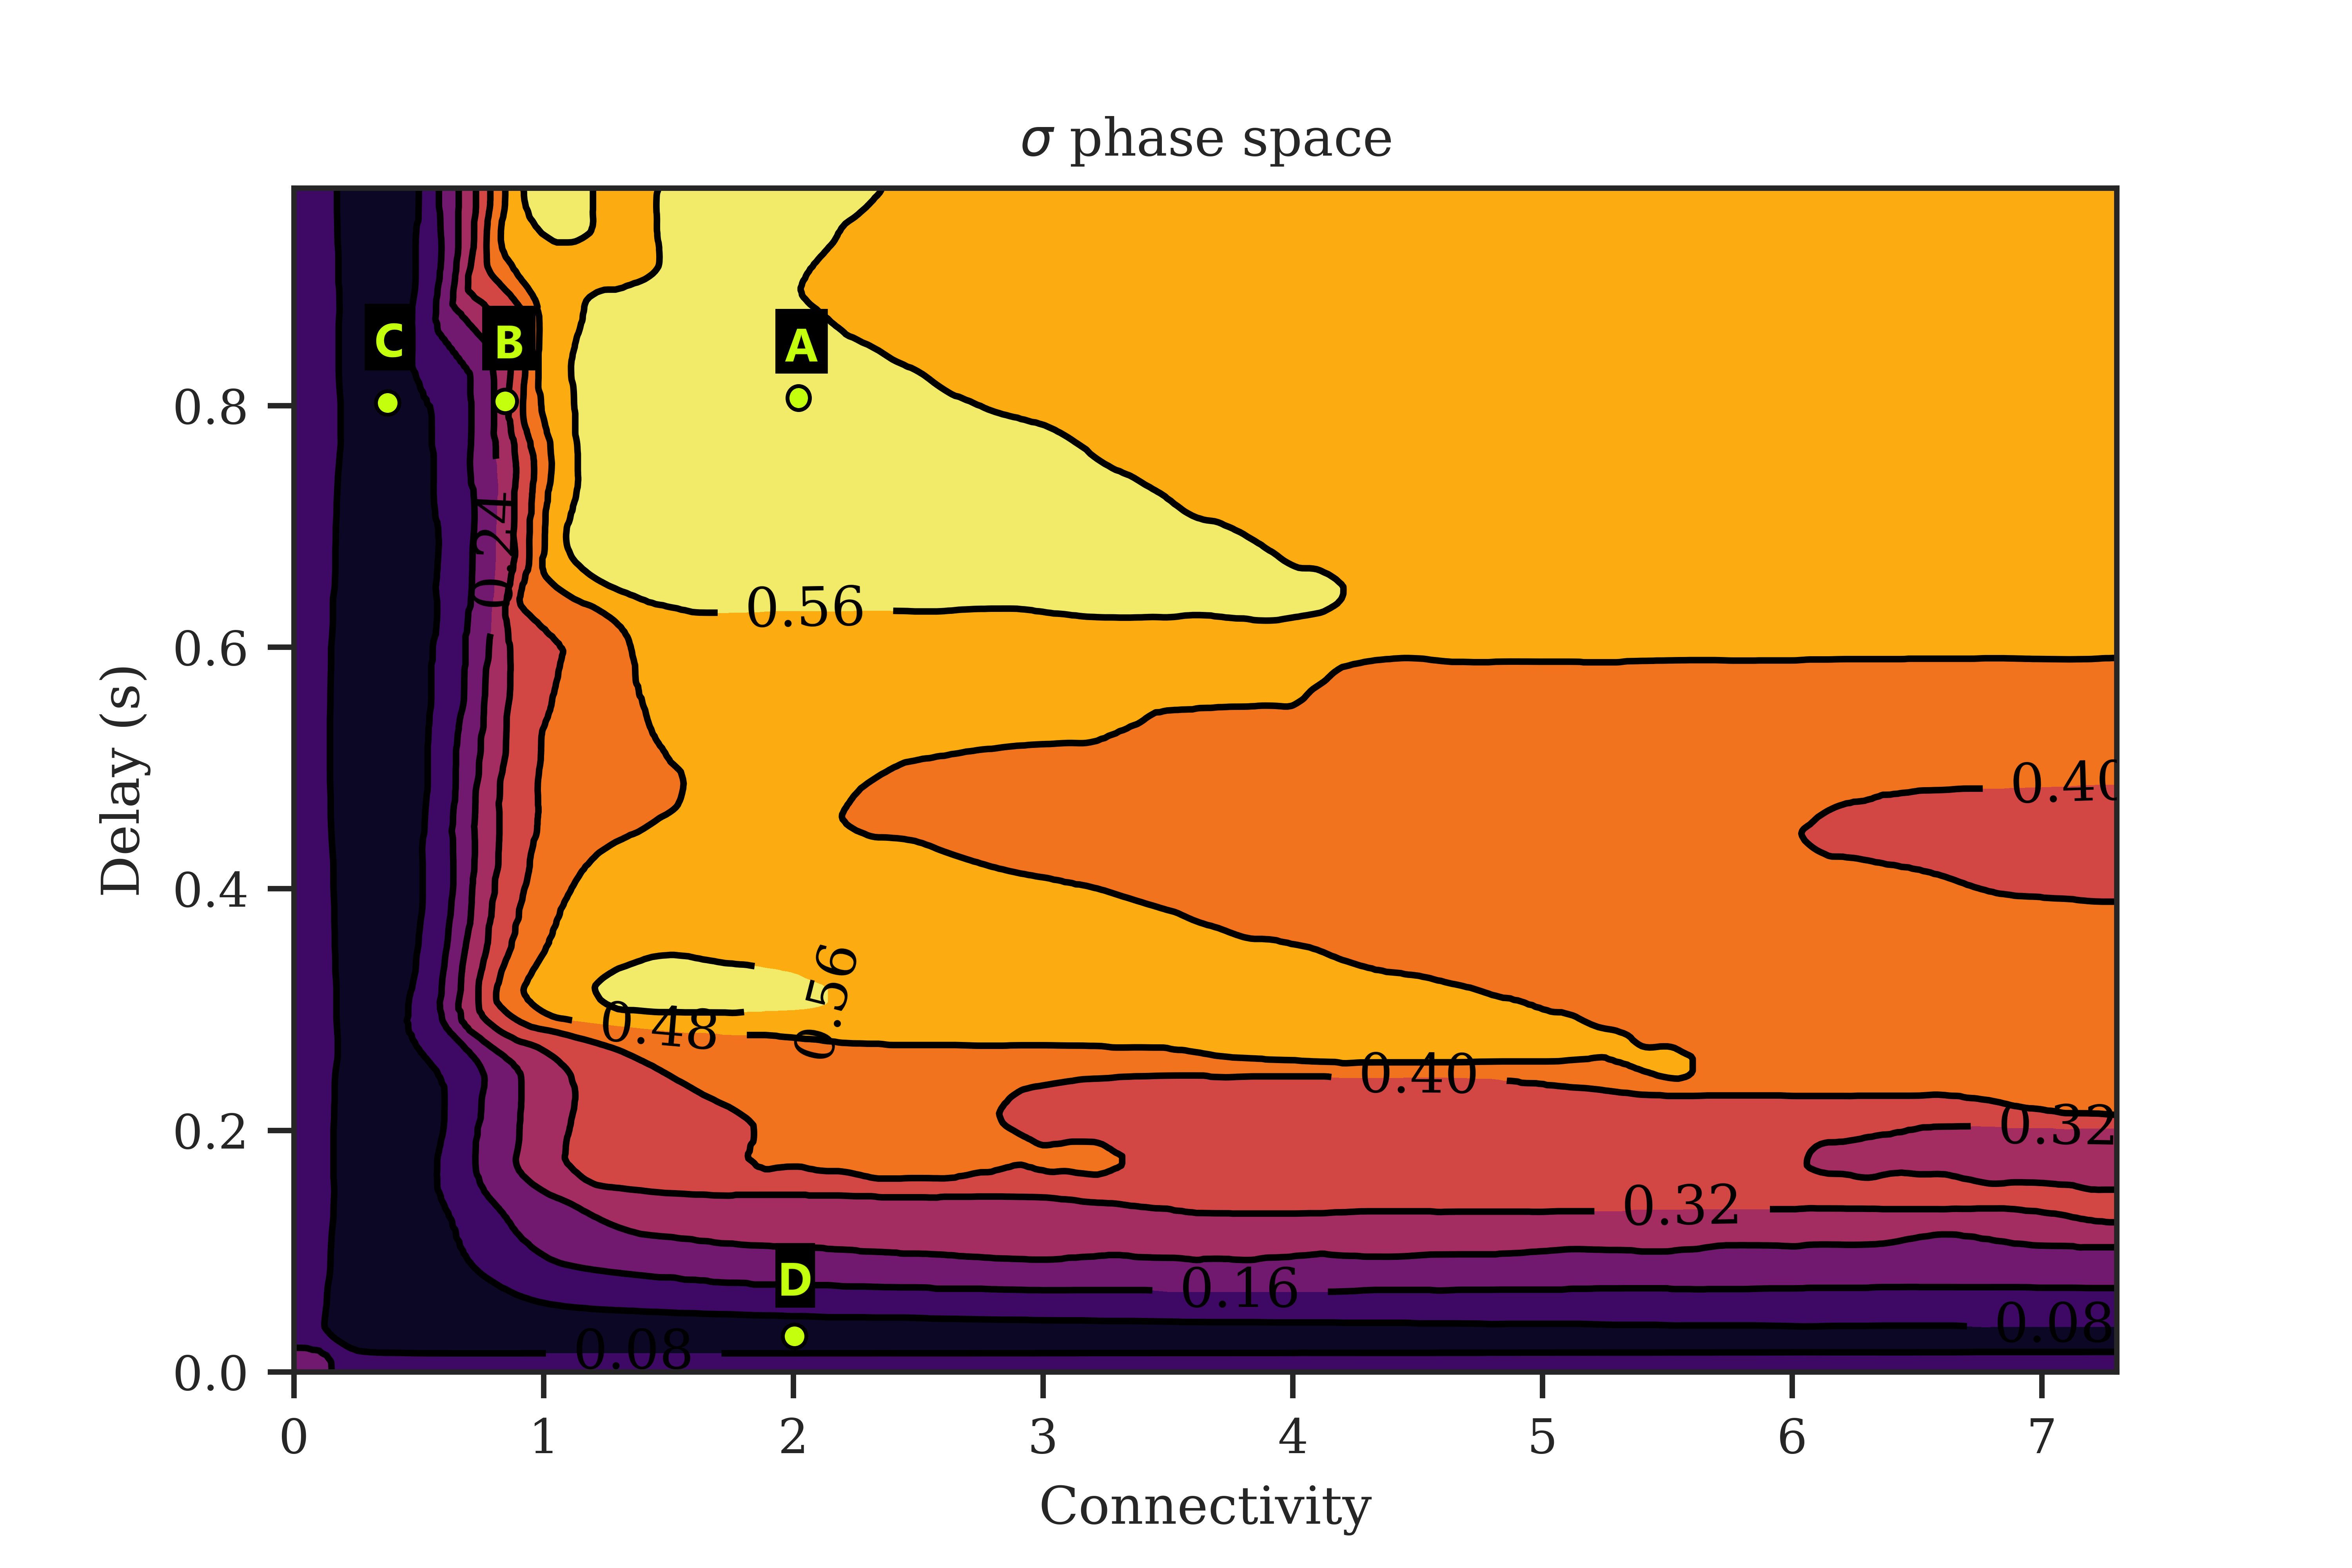
\includegraphics[width = \textwidth]{Figures/animation_chapter/IF_sigma_phase_space_contour_selected_points.png}
	\caption{
		نقاط انتخاب شده در فضای فاز شبکه‌ی نورون‌های انباشت‌وشلیک.
	}
	\label{fig:IF_abc}
	\end{subfigure}
	\hfill
	\begin{subfigure}{0.5\textwidth}
		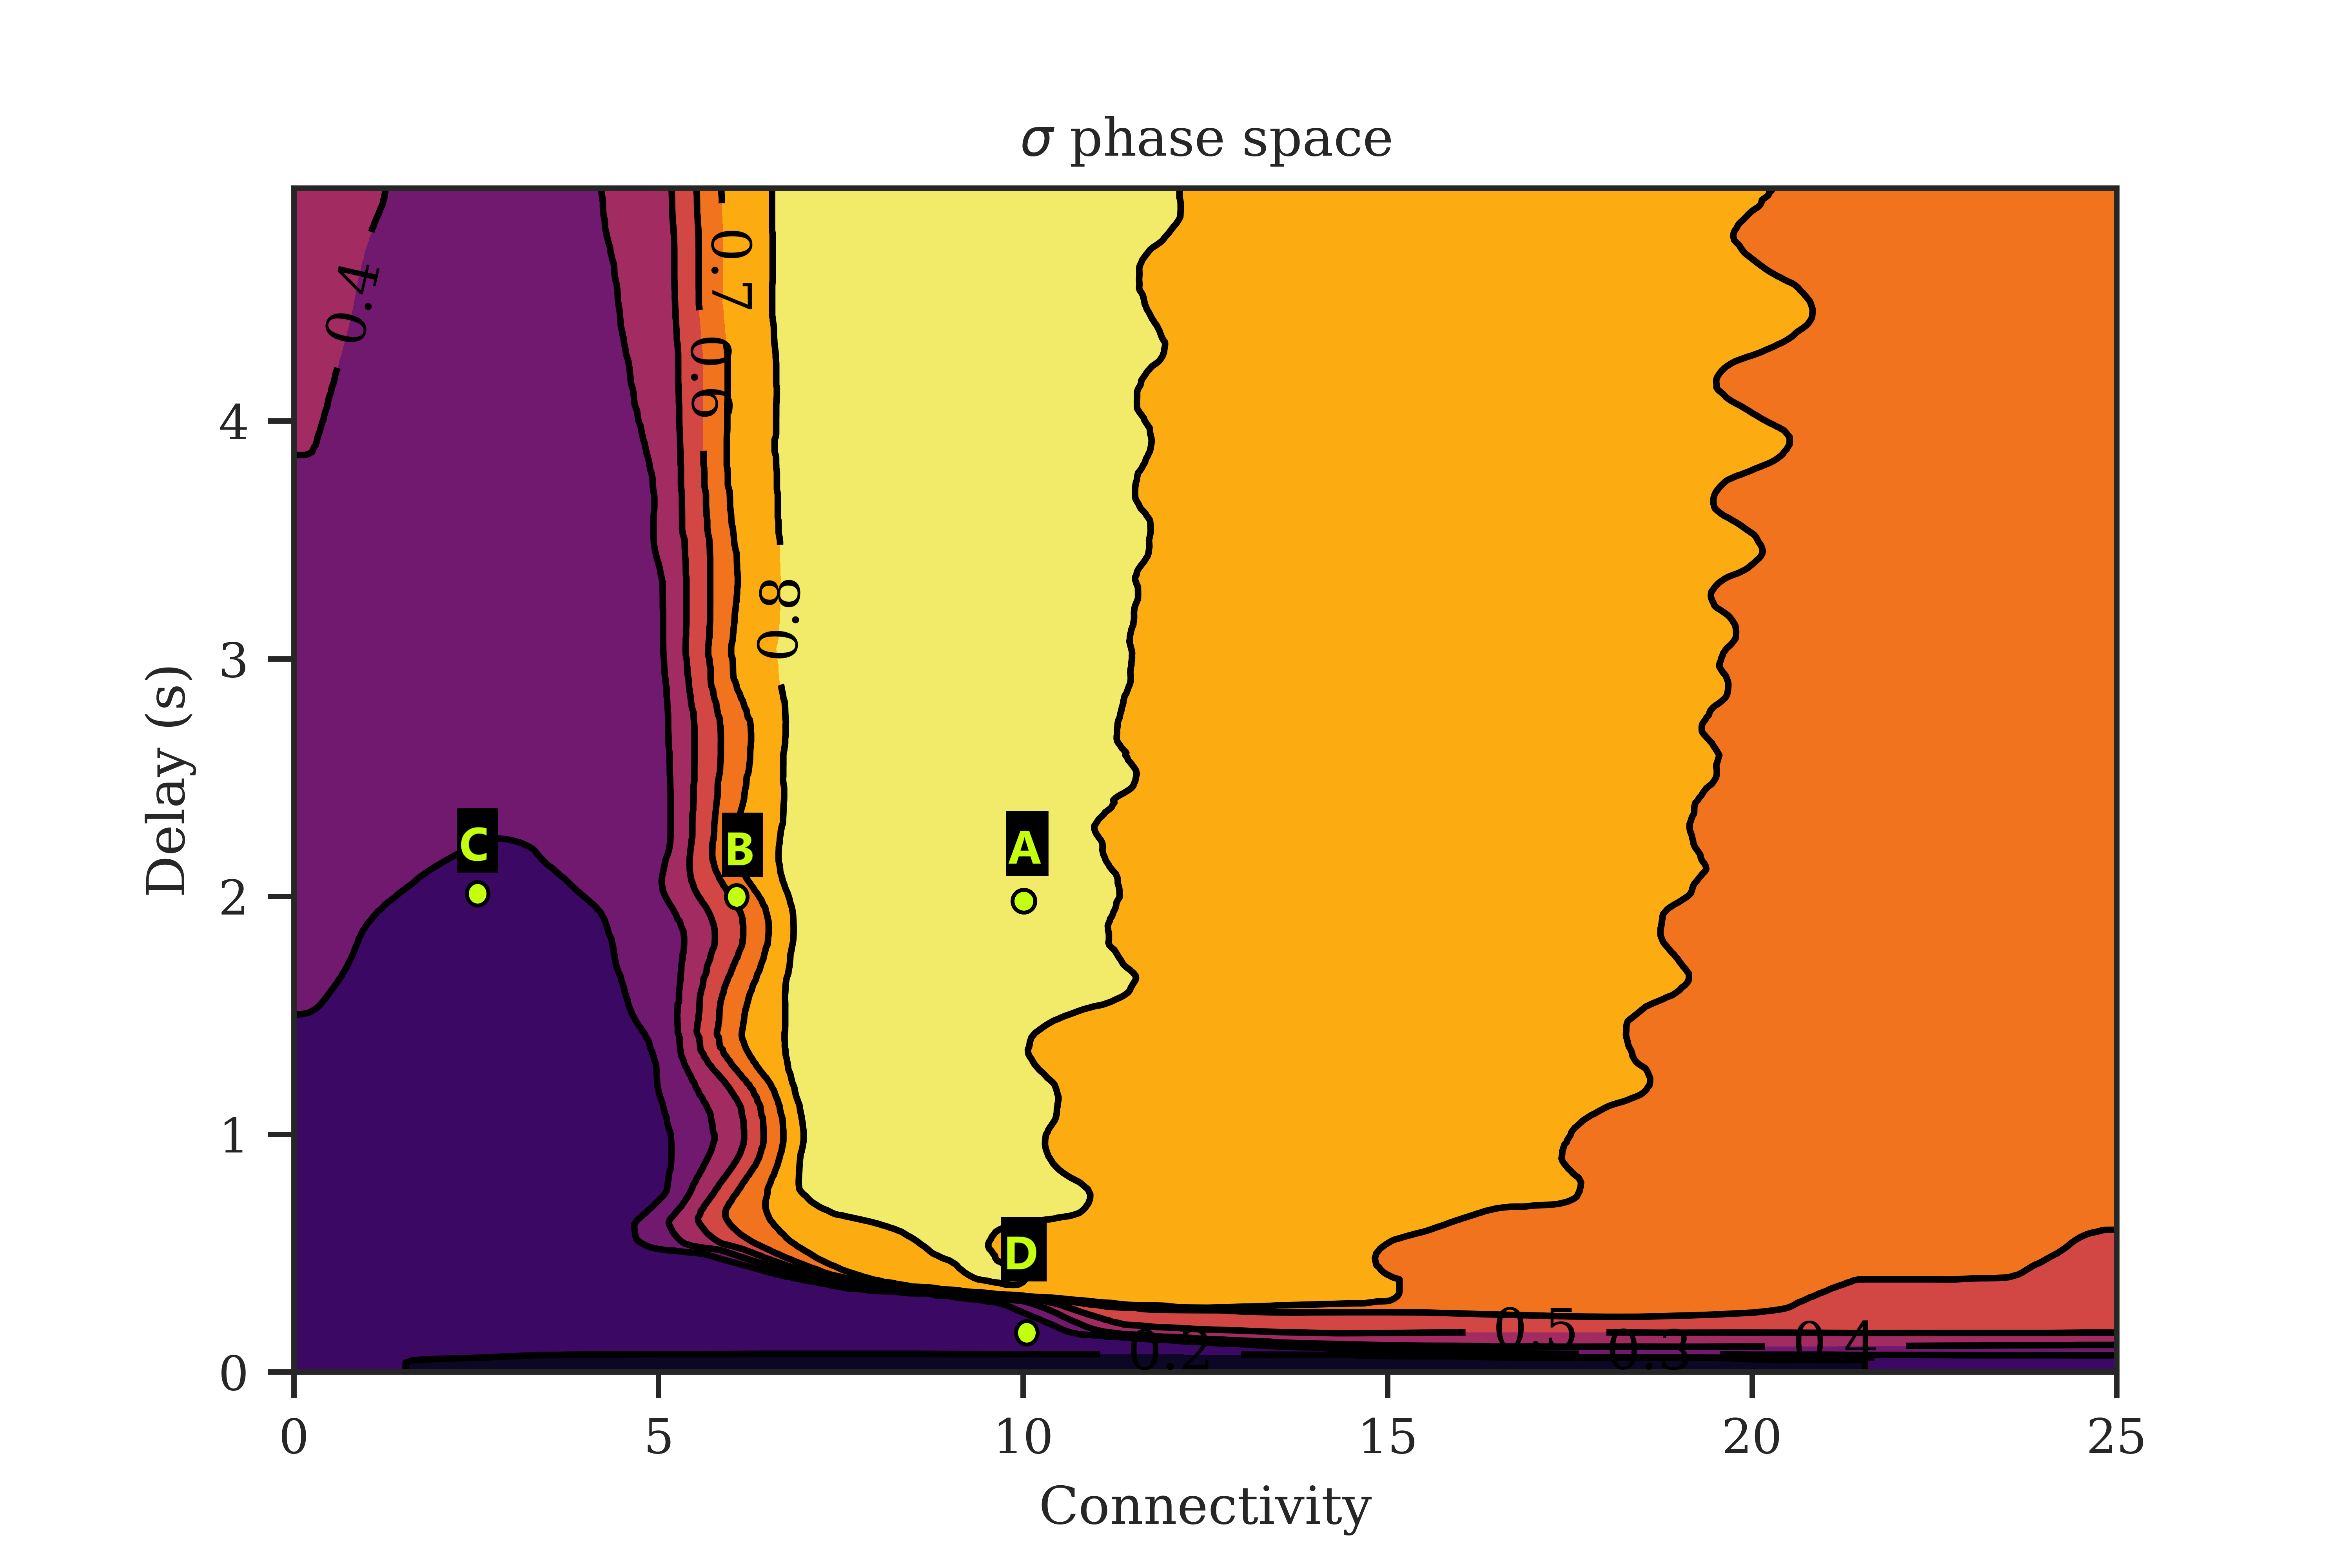
\includegraphics[width = \textwidth]{Figures/animation_chapter/Rotational_sigma_phase_space_contour_selected_points.png}
		\caption{
		نقاط انتخاب شده در فضای فاز شبکه‌ی نورون‌های چرخنده.
	}
		\label{fig:Rotational_abc}
	\end{subfigure}
	\hfill
	\begin{subfigure}{0.5\textwidth}
		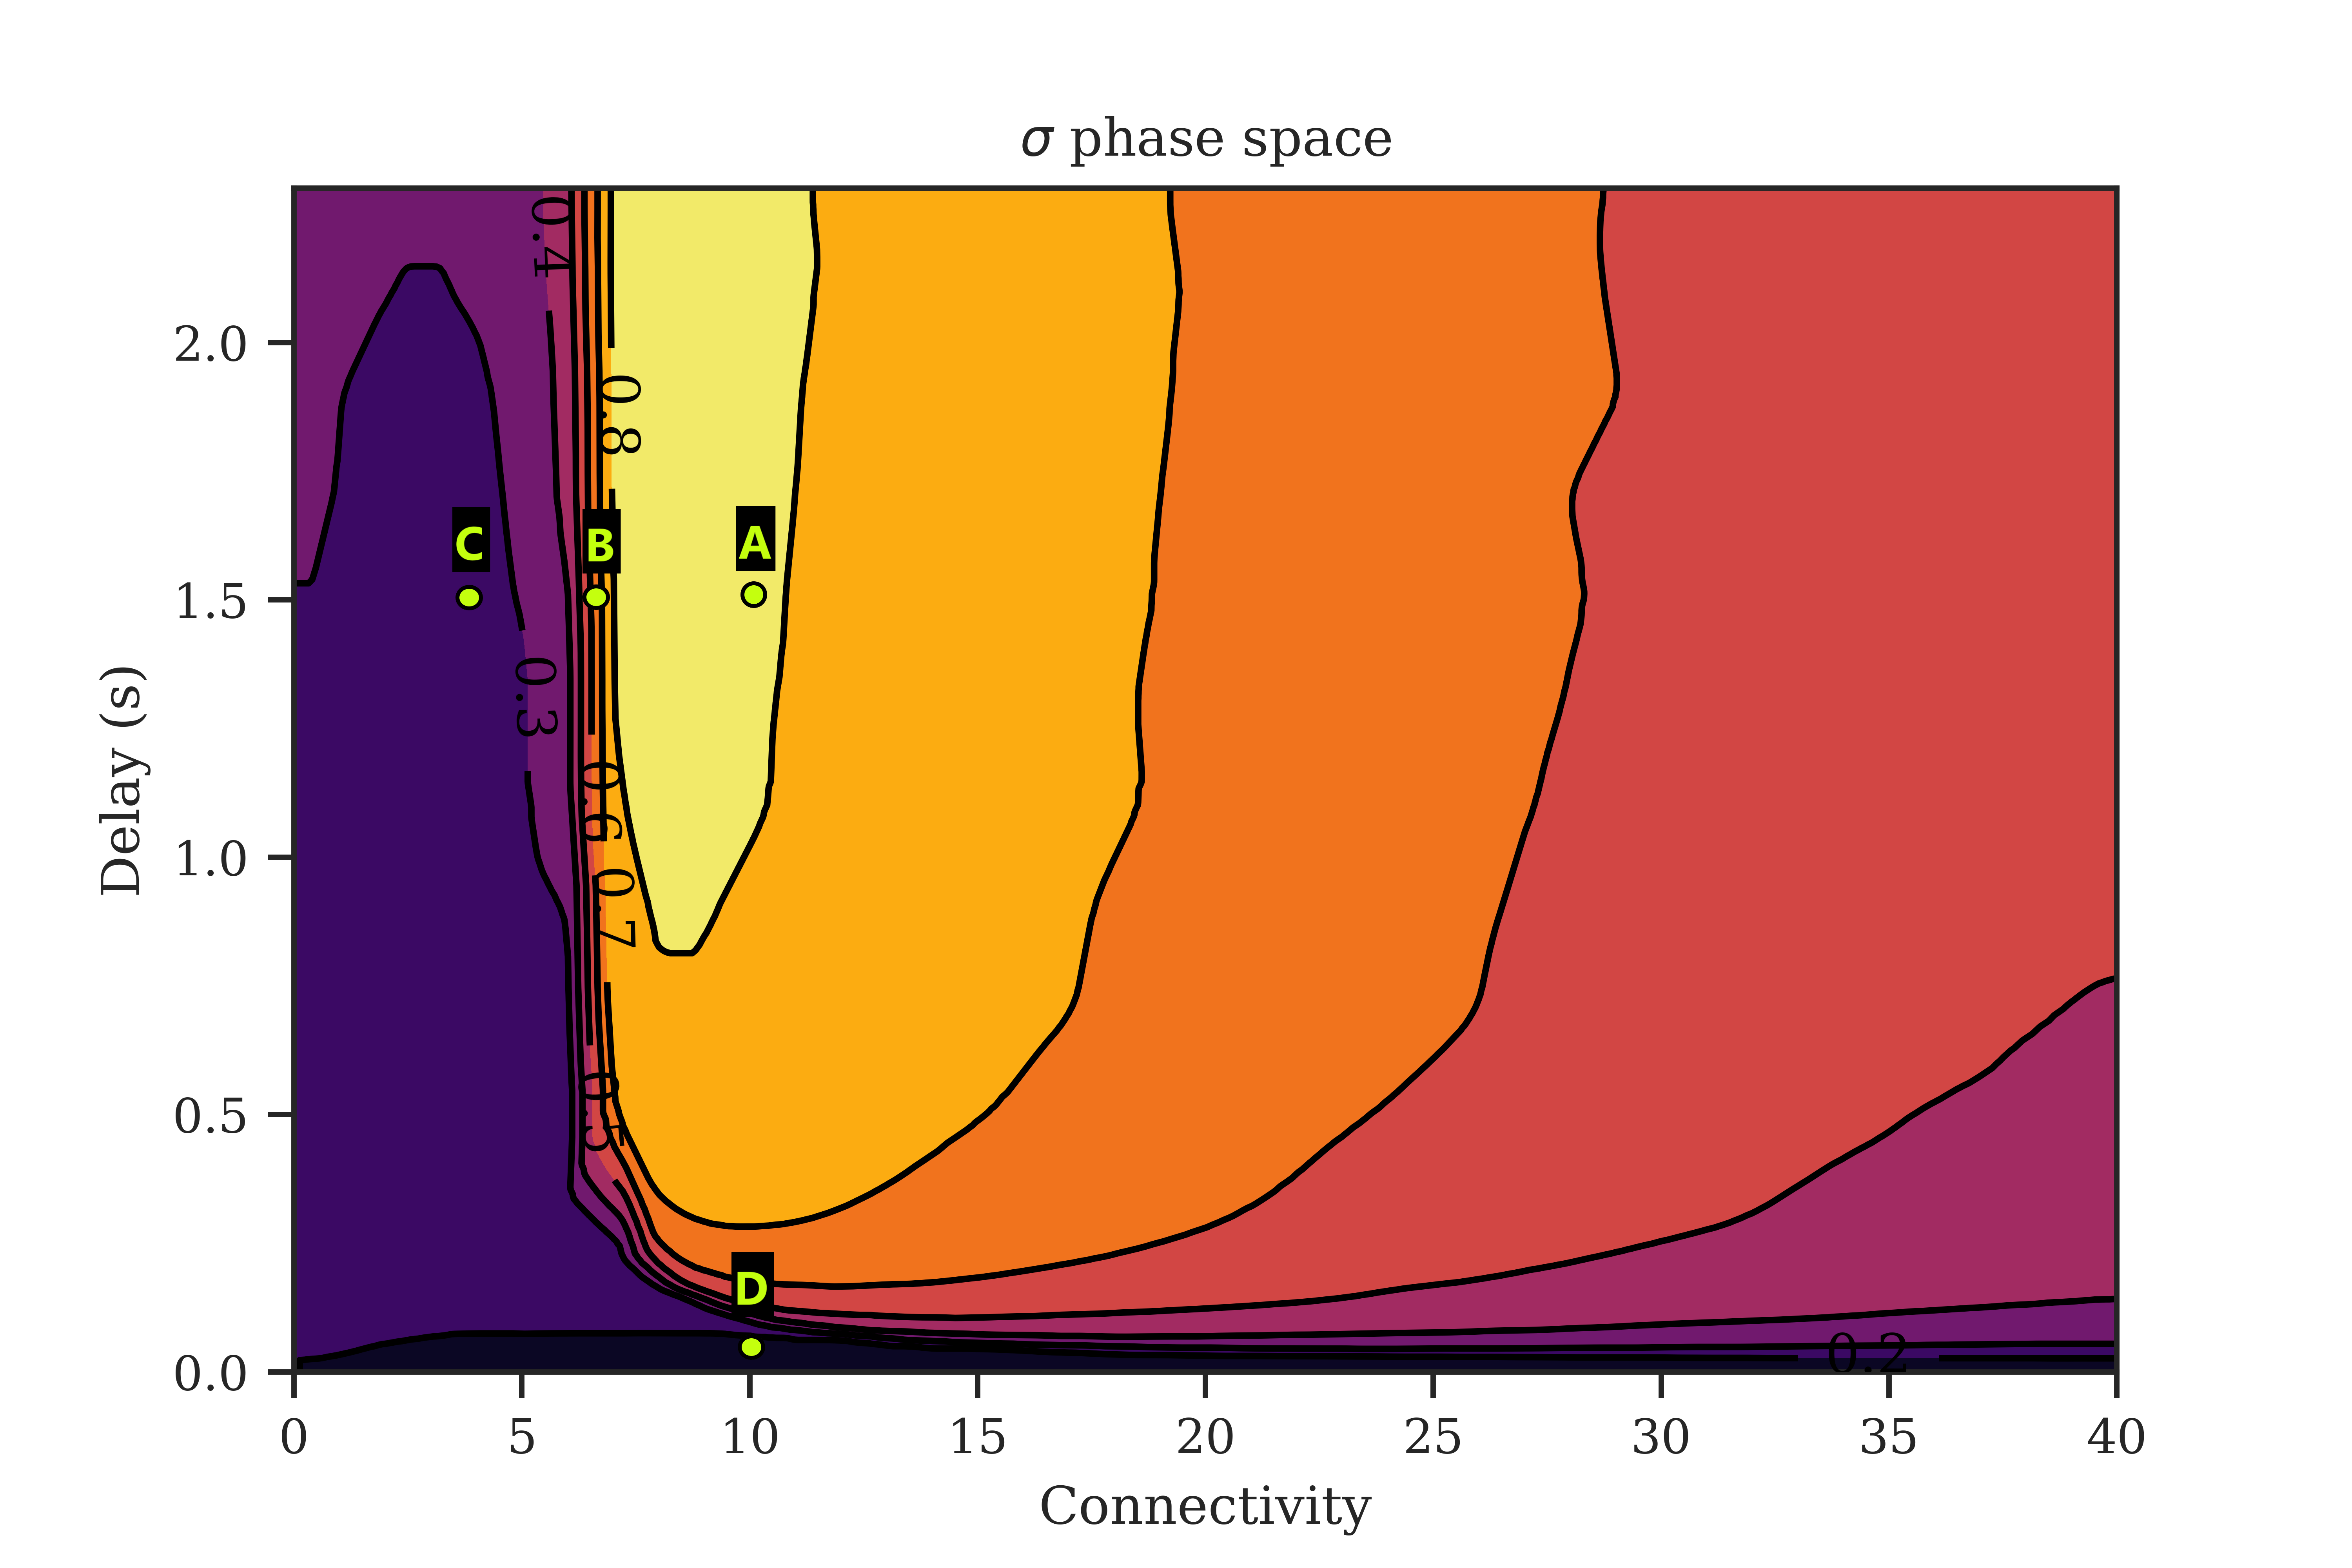
\includegraphics[width = \textwidth]{Figures/animation_chapter/Non_repulsive_sigma_phase_space_contour_alpha20_selected_points.png}
		\caption{
		نقاط انتخاب شده در فضای فاز شبکه‌ی نورون‌های ساده.
		}
		\label{fig:Non_repulsive_abc}
	\end{subfigure}
	\hfill
	\caption{
	نقطه‌ی 
A
:معرف نقطه‌ای است که سامانه دقیقا در حالت هم‌گام قرار دارد.
نقطه‌ی
B
:نقطه‌ای میانی بین فاز هم‌گام و ناهم‌گام است.
نقطه‌ی
C
: حالتی ناهم‌گام است با این وجود که تاخیر آکسونی در سامانه وجود دارد اما هم‌گامی رخ نمی‌دهد.
D
: حالتی از سامانه است که ضریب تاثیر قابل ملاحظه‌ای دارد اما تاخیر در سامانه نزدیک به صفر است.}
	\label{fig:abc_points_neuron_models}
\end{figure}

\newpage

\قسمت{پویانمایی}
\زیرقسمت{مدل انباشت‌وشلیک}
شکل
\ref{fig:IF_animation_A}
نمایی از ۶ برداشت از پویانمایی سامانه‌ی نورون‌های انباشت‌وشلیک ارائه شده است. شرایط اولیه این سامانه به گونه‌ای است که همه‌ی نورون‌ها در فضای فاز به صورت یکنواخت توزیع شده‌اند. تو گویی حالت اولیه شبکه یک مستطیل یکنواخت را روایت می‌کرده است.\\
بیاید ورقی بزنیم و به نکاتی این زنجیره از اشکال با خود دارد بپردازیم:
\begin{description}
	\item[تجمع فازها] 
	نمای سامانه در این حالت بسیار قابل توجه است. همه‌ی نورون‌هایی که جریان خارجی مشخصی دارند؛ در یک فاز جمع شده‌اند.
	\item[نورون‌های همسایه] 
	 فاصله‌ی فاز هر دو نورون با جریان خارجی نزدیک به هم رابطه‌ای خطی دارد. این پیشامد نیز با بازنویسی معادلات دیفرانسیل قابل درک است.
	 \begin{align}
	 	\dot{v_a} &= a - v_a - g E ,\\
	 	\Delta\dot{v_a} &= \Delta a - \Delta v_a ,\\
	 	\frac{\Delta\dot{v_a}}{\Delta a} &= 1 - \frac{\Delta v_a}{\Delta a}\\
		\frac{\Delta v_a}{\Delta a} &= 1 + C_0 e^{-t}\\
		\frac{\Delta v_a}{\Delta a} &\rightarrow 1 .
	 \end{align}
 پس این معادلات کاملا توضیح می‌دهد که فارغ از شرط اولیه در صفحه‌ی فاز باید انتظار یک خط با شیب یک داشته باشیم که همه‌ی نورون‌ها در آن جمع شده‌اند. در کنار این شرط دوره‌ای هم باید در نظر گرفته شود که باعث شده است این خط بریده‌بریده شود.
 	\item[جفت شدن سرعت‌ها]
 	هم‌گامی در این شکل به معنای جفت شدن سرعت‌های نورون‌ها با یکدیگر است و نه فاز آن‌ها. آن‌ها با هم به سمت آستانه حرکت می‌کنند و باهم عقب‌نشینی می‌کنند اما دوشادوش یک‌دیگر کمتر قرار می‌گیرند.\\
 	بیاید به معادلات قسمت قبل دوباره نگاه کنیم. می‌توانیم نتیجه بگیریم تفاوت سرعت‌های دو نورون با جریان‌های پشت سرهم صفر خواهد بود.
 	\begin{align}
 		\Delta\dot{v_a} &= \Delta a - \Delta v_a\\
 		&= \Delta a \big(1 - \frac{\Delta v_a}{\Delta a} \big) \rightarrow 0 .
 	\end{align}
 	به این ترتیب می‌توان فهمید این فازها نیستند که باهم جفت می‌شوند 
 	($\Delta v_a \nrightarrow 0 $)
 	بلکه این سرعت‌ها هستند که بهم قفل می‌شوند
 	($\Delta \dot{v_a} \rightarrow 0 $).
\end{description}

\newpage
\begin{figure}[!h]
	\begin{subfigure}{0.5\textwidth}
		\includegraphics[width = \textwidth]{../scripts/all_neurons_model_in_one_place/animations/sea_shore/black_white/IF_frames/A/1.png}
		\caption{
			ثانیه صفرم		
		}
		%		\label{}
	\end{subfigure}
	\hfill
	\begin{subfigure}{0.5\textwidth}
		\includegraphics[width = \textwidth]{../scripts/all_neurons_model_in_one_place/animations/sea_shore/black_white/IF_frames/A/50.png}
		\caption{
			ثانیه $0.5$
		}
		%		\label{}
	\end{subfigure}
	\hfill
	\begin{subfigure}{0.5\textwidth}
		\includegraphics[width = \textwidth]{../scripts/all_neurons_model_in_one_place/animations/sea_shore/black_white/IF_frames/A/100.png}
		\caption{
			ثانیه $1$		
		}
		%		\label{}
	\end{subfigure}
	\hfill
	\begin{subfigure}{0.5\textwidth}
		\includegraphics[width = \textwidth]{../scripts/all_neurons_model_in_one_place/animations/sea_shore/black_white/IF_frames/A/150.png}
		\caption{
			ثانیه $1.5$
		}
		%		\label{}
	\end{subfigure}
	\hfill
	\begin{subfigure}{0.5\textwidth}
		\includegraphics[width = \textwidth]{../scripts/all_neurons_model_in_one_place/animations/sea_shore/black_white/IF_frames/A/200.png}
		\caption{
			ثانیه $2$
		}
		%		\label{}
	\end{subfigure}
	\hfill
	\begin{subfigure}{0.5\textwidth}
		\includegraphics[width = \textwidth]{../scripts/all_neurons_model_in_one_place/animations/sea_shore/black_white/IF_frames/A/250.png}
		\caption{
			ثانیه $2.5$
		}
		%		\label{}
	\end{subfigure}
	\hfill
	\caption{
		نمایی از پویایی سامانه‌ی نورونی انباشت‌وشلیک در نقطه‌ی A - این پویانمایی پس از گذشت ۲۰۰ ثانیه از تاریخچه‌ی سامانه انجام شده است. شرایط اولیه به گونه‌ای است که نورون‌ها با توزیع یکنواخت در صفحه‌ی فاز پراکنده شده‌اند.}
	\label{fig:IF_animation_A}
\end{figure}
\newpage
\زیرقسمت{مدل چرخنده}
شکل
\ref{fig:rotational_animation_A}
نمایی از ۶ برداشت از پویانمایی سامانه‌ی نورون‌های ساده ارائه شده است. شرایط اولیه این سامانه به گونه‌ای است که همه‌ی نورون‌ها در فضای فاز به صورت یکنواخت توزیع شده‌اند. تو گویی حالت اولیه شبکه یک مستطیل یکنواخت را روایت می‌کرده است.\\

\begin{description}
	\item[تشابهات]
	به نظر می‌آید نکاتی که مربوط به حالت هم‌گامی در قسمت انباشت‌وشلیک روایت کردیم (به جز ویژگی‌هایی جزئی) برای این سامانه هم برقرار است. 
	\item[منحنی جاذب] 
	توجه داشته باشیم که در برخی از قسمت‌های شکل، نورون‌ها روی منحنی‌هایی تجمع کرده‌اند. این منحنی‌ها را می‌توان با نوشتن معادلات توصیف کرد:
	 \begin{align}
		\dot{\theta_a} &= a - \cos\theta_a - g E ,\\
		\Delta\dot{\theta_a} &= \Delta a - \Delta \cos\theta_a ,\\
		\frac{\Delta\dot{v_a}}{\Delta a} &= 1 - \sin\theta_a\frac{\Delta \theta_a}{\Delta a},\\
		\frac{\Delta\dot{v_a}}{\Delta a} &= 0 : 1 - \sin\theta_a\frac{\Delta \theta_a}{\Delta a} = 0\\
		\Delta \theta &= - \frac{\Delta a}{\sin\theta}\\
		&= - cosec \theta_a \Delta a.
	\end{align}
همان طور که معادلات نشان می‌دهد منحنی‌های تجمع بسیار شبیه به عکس سینوس هستند. 
	\item[پراکندگی در اطراف منحنی]
	شاید بپرسیم که چرا در ناحیه‌های دیگر صفحه‌ی فاز چرا نورون‌ها تجمع نکرده‌اند. می‌تواند به این علت باشد که منحنی‌های یاد شده به ازای آن جریان‌های خارجی جاذب نیستند. هر چند حضور شرط دوره‌ای نیز بی‌تاثیر نیست.
\end{description}


\newgeometry{top=5mm, bottom=5mm}
\begin{figure}
	\begin{subfigure}{0.5\textwidth}
		\includegraphics[width = \textwidth]{../scripts/all_neurons_model_in_one_place/animations/sea_shore/black_white/Rotational_frames/A/250.png}
		\caption{
			ثانیه صفرم		
		}
		%		\label{}
	\end{subfigure}
	\begin{subfigure}{0.5\textwidth}
		\includegraphics[width = \textwidth]{../scripts/all_neurons_model_in_one_place/animations/sea_shore/black_white/Rotational_frames/A/300.png}
		\caption{
			ثانیه $0.5$
		}
		%		\label{}
	\end{subfigure}
	\begin{subfigure}{0.5\textwidth}
		\includegraphics[width = \textwidth]{../scripts/all_neurons_model_in_one_place/animations/sea_shore/black_white/Rotational_frames/A/350.png}
		\caption{
			ثانیه $1$		
		}
		%		\label{}
	\end{subfigure}
	\begin{subfigure}{0.5\textwidth}
		\includegraphics[width = \textwidth]{../scripts/all_neurons_model_in_one_place/animations/sea_shore/black_white/Rotational_frames/A/400.png}
		\caption{
			ثانیه $1.5$
		}
		%		\label{}
	\end{subfigure}
	\begin{subfigure}{0.5\textwidth}
		\includegraphics[width = \textwidth]{../scripts/all_neurons_model_in_one_place/animations/sea_shore/black_white/Rotational_frames/A/450.png}
		\caption{
			ثانیه $2$
		}
		%		\label{}
	\end{subfigure}
	\begin{subfigure}{0.5\textwidth}
		\includegraphics[width = \textwidth]{../scripts/all_neurons_model_in_one_place/animations/sea_shore/black_white/Rotational_frames/A/500.png}
		\caption{
			ثانیه $2.5$
		}
		%		\label{}
	\end{subfigure}
	\begin{subfigure}{0.5\textwidth}
		\includegraphics[width = \textwidth]{../scripts/all_neurons_model_in_one_place/animations/sea_shore/black_white/Rotational_frames/A/550.png}
		\caption{
			ثانیه $3$
		}
		%		\label{}
	\end{subfigure}
	\begin{subfigure}{0.5\textwidth}
		\includegraphics[width = \textwidth]{../scripts/all_neurons_model_in_one_place/animations/sea_shore/black_white/Rotational_frames/A/600.png}
		\caption{
			ثانیه $3.5$
		}
		%		\label{}
	\end{subfigure}
	\caption{
		نمایی از پویایی سامانه‌ی نورونی چرخنده در نقطه‌ی A - این پویانمایی پس از گذشت ۲۰۰ ثانیه از تاریخچه‌ی سامانه انجام شده است. با شرایط اولیه‌ای که نورون‌ها با توزیع یکنواخت در صفحه‌ی فاز پراکنده شده‌اند.	
	}
	\label{fig:rotational_animation_A}
\end{figure}
\restoregeometry 

\newpage
\زیرقسمت{مدل نورونی ساده}
در شکل 
\ref{fig:simple_animation_A}
نمایی از ۶ برداشت از پویانمایی سامانه‌ی نورون‌های ساده ارائه شده است. شرایط اولیه این سامانه به گونه‌ای است که همه‌ی نورون‌ها در فضای فاز به صورت یکنواخت توزیع شده‌اند. تو گویی حالت اولیه شبکه یک مستطیل یکنواخت را روایت می‌کرده است.\\
این پویانمایی نشانی‌های بسیار خوبی به ما می‌دهد تا در بخش‌های بعدی هم‌گامی را به شکل تحلیلی نیز توضیح دهیم. شاید این واضح‌ترین تصویری است که می‌توانیم در مورد شکل‌گیری همگامی در میان شبکه نورونی خود ببینیم.
\begin{description}
	\item[منحنی جاذب؟]
	چون این مدل جمله‌ای از جنس مهار ذاتی درون معادلات دیفرانسیل خود ندارد؛ شکل نهایی آن دارای منحنی جاذب نیست و چگالی یک یکنواختی دارد.
	\item[مرزهای سامانه]
	در هر مرحله از فراز و فرود سامانه، شکل مستطیلی آن تبدیل به متوازی‌الاضلاع می‌شود و پس از عبور از آستانه، شرط دوره‌ای شکل اولیه آن را به او برمی‌گرداند.
	\item[شروع هم‌گامی]
	به نظر می‌آید شروع هم‌گامی از ضریب تاثیری است که موفق می‌شود نورون‌هایی که کمترین جریان خارجی را دارند از محور آستانه پس بزند. به طوری که در چند لحظه‌ی متوالی از تیزه زدن باز بمانند.
	\item[مرزبندی مشابه]
	اگر به مرزهای فضای حالت‌های نورون‌های چرخنده و انباشت‌وشلیک توجه کنیم؛ متوجه می‌شویم که آن‌ها نیز زیرشکلی از این مستطیل را در اختیار داشتند و تحول آن‌ها از ناهم‌گامی به هم‌گامی باید شبیه شکل نورون‌های ساده باشد. 
\end{description}

\newpage
\begin{figure}
	\begin{subfigure}{0.5\textwidth}
		\includegraphics[width = \textwidth]{../scripts/all_neurons_model_in_one_place/animations/sea_shore/black_white/Non_repulsive_frames/A/1.png}
		\caption{
			ثانیه صفرم		
		}
		%		\label{}
	\end{subfigure}
	\hfill
	\begin{subfigure}{0.5\textwidth}
		\includegraphics[width = \textwidth]{../scripts/all_neurons_model_in_one_place/animations/sea_shore/black_white/Non_repulsive_frames/A/50.png}
		\caption{
			ثانیه $0.5$
		}
		%		\label{}
	\end{subfigure}
	\hfill
	\begin{subfigure}{0.5\textwidth}
		\includegraphics[width = \textwidth]{../scripts/all_neurons_model_in_one_place/animations/sea_shore/black_white/Non_repulsive_frames/A/100.png}
		\caption{
			ثانیه $1$		
		}
		%		\label{}
	\end{subfigure}
	\hfill
	\begin{subfigure}{0.5\textwidth}
		\includegraphics[width = \textwidth]{../scripts/all_neurons_model_in_one_place/animations/sea_shore/black_white/Non_repulsive_frames/A/150.png}
		\caption{
			ثانیه $1.5$
		}
		%		\label{}
	\end{subfigure}
	\hfill
	\begin{subfigure}{0.5\textwidth}
		\includegraphics[width = \textwidth]{../scripts/all_neurons_model_in_one_place/animations/sea_shore/black_white/Non_repulsive_frames/A/200.png}
		\caption{
			ثانیه $2$
		}
		%		\label{}
	\end{subfigure}
	\hfill
	\begin{subfigure}{0.5\textwidth}
		\includegraphics[width = \textwidth]{../scripts/all_neurons_model_in_one_place/animations/sea_shore/black_white/Non_repulsive_frames/A/250.png}
		\caption{
			ثانیه $2.5$
		}
		%		\label{}
	\end{subfigure}
	\hfill
	\caption{
		نمایی از پویایی سامانه‌ی نورونی ساده در نقطه‌ی A - این پویانمایی پس از گذشت ۲۰۰ ثانیه از تاریخچه‌ی سامانه به ازای شرایط اولیه یکنواخت توزیع نورون‌ها در صفحه‌ی فاز.	
	}
	\label{fig:simple_animation_A}
\end{figure}

\قسمت{جمع‌بندی}
همان‌طور که انتظار می‌رفت تصویرسازی کمک شایانی در فهم سامانه‌ها به ما ارائه داد و باعث شد تفاوت‌ها و شباهت‌های زیادی را بین سامانه‌ها دریافت کنیم. از مهم‌ترین شباهت‌هایی که بین مدل‌های نورونی پیدا کردیم؛ «جفت‌شدن سرعت‌ها» و «مرزهای مستطیل‌گون» اهمیت بسیار زیادی دارند. زیرا به نظر می‌آيد که هم‌گامی ارتباط نزدیکی با هر کدام از این خواص دارد و شاید اصلا ناشی از این دو اتفاق هندسی باشد.\\
از آن‌جا که مدل نورونی ساده در این دو خاصیت با مدل‌های قبلی شباهت دارد و هم‌چنین خاصیت هم‌گامی را به قوت همراه خود دارد؛ اجازه دهید تا محاسبات تحلیلی خود را با آن آغاز کنیم. باشد که راهنمایی برای تحلیل مدل‌های دیگر نیز پیدا کنیم.














\section*{فرصتی برای مدل‌های دیگر نورونی}
در بخش قبل به بررسی ویژگی‌های مدل انباشت‌-شلیک پراختیم. اگر چه این مدل بسیار ساده توانست رفتارهای آشنایی را برای ما بازتولید کند اما شامل محدودیت‌هایی است. این محدودیت‌ها باعث می‌شود تا ما به سراغ مدل‌های نورونی دیگری مانند نورون‌های چرخنده برویم.\\
این مدل نسبت به مدل قبلی شامل ویژگی‌های مثبتی است. یکی از ویژگی‌های خوب آن این است که پس از بازنشانی فاز نورون تیزه زده، فاز آن به زاویه‌ای برده می‌شود که دارای خواص مثلثاتی مشابهی است. به این معنا که دیگر شاهد گسستگی در اندازه‌ی جملاتی که تحول نورون را توصیف می‌کنند؛ نیستیم.\\
%\section*{فرصتی برای مدل‌های دیگر نورونی}
در بخش قبل به بررسی ویژگی‌های مدل انباشت‌-شلیک پراختیم. اگر چه این مدل بسیار ساده توانست رفتارهای آشنایی را برای ما بازتولید کند اما شامل محدودیت‌هایی است. این محدودیت‌ها باعث می‌شود تا ما به سراغ مدل‌های نورونی دیگری مانند نورون‌های چرخنده برویم.\\
این مدل نسبت به مدل قبلی شامل ویژگی‌های مثبتی است. یکی از ویژگی‌های خوب آن این است که پس از بازنشانی فاز نورون تیزه زده، فاز آن به زاویه‌ای برده می‌شود که دارای خواص مثلثاتی مشابهی است. به این معنا که دیگر شاهد گسستگی در اندازه‌ی جملاتی که تحول نورون را توصیف می‌کنند؛ نیستیم.\\

\فصل{شبکه‌ی نورون‌های چرخنده}
\label{chap:rotational}
در این مدل به جای آن که برای شبکه خود از مدل انباشت-شلیک استفاده کنیم از مدل چرخنده استفاده می‌کنیم. در این مدل نورون‌های ما مانند دونده‌هایی به دور دایرهٔ مثلثاتی می‌دوند. ما نقطه‌ی فاز $\pi$ را به عنوان علامت برای این دونده‌ها قرار دادیم. هر زمان که دونده‌ای از علامت خود گذشت یک تیزه برای او درنظرمی‌گیریم و بلافاصله او را به فاز $-\pi$ باز می‌گردانیم.\\

برای توصیف فاز هر نورون از معادلات زیر استفاده می‌کنیم:
\begin{tcolorbox}
	\begin{equation}
		\begin{cases}
			\dot{\theta_i}=I_i - \cos{\theta_i} - g E, \hspace{2ex} \theta_i \leq \pi \\
			\dot{E} = M - \alpha E\\
			\dot{M} = -  \alpha M + \frac{ \alpha^{2} }{N} \sum_{n|t_{n}<t} \delta(t - t_n - t_d)
		\end{cases}
	\end{equation}
	\begin{enumerate}[-]
		\item $\theta_i$:
		مشخص کننده‌ی فاز هر نورون. این فاز میان دو لبه در حال حیات است. کوچکترین کران بالای آن همان حالت آستانه در $\pi$ است و بزرگترین کران پایین آن نگه‌دارنده‌ای است که از ریزش نورون‌ها جلوگیری می‌کند.
		\item $E$:
		میدانی است که شدت فعالیت شبکه را نشان می‌دهد.
		\item $M$:
		یک پارامتر فرعی که در حل معادله دیفرانسیل مرتبه دوم به دو معادلهٔ تحول مرتبه اول ما را یاری کرده است.
	\end{enumerate}
\end{tcolorbox}

\قسمت{آهنگ تیزه زدن}
برای نورونی تنها که پویایی از جنس چرخنده دارد؛ دوره‌ی تناوب و بسامد تیزه زدن آن برحسب مجموع جریان ورودی‌ رفتاری مطابق زیر دارد (پیوست
\ref{appendix:activity_calculation}):

\begin{align}
	T &= \frac{2\pi}{\sqrt{I^2 - 1}},\\
	f &= \frac{1}{T} = \frac{\sqrt{I^2 - 1}}{2\pi}.
\end{align}
این به این معناست که مدل چرخنده و انباشت‌وشلیک اگر چه هر دو با افزایش جریان، بسامد تیزه زدنشان افزایش می‌یابد اما رفتار تغییر آن به دو گونه‌ی متفاوت صورت می‌پذیرد. این نکته‌ی مهمی است که در هنگام مقایسه‌ی دو مدل باید به خاطر داشته باشیم.

\قسمت{نشانگر توسعه یافته‌ی تشخیص همگامی}
گفتنی است که برای تشخیص هم‌گامی می‌توان پارامترهای دیگری نیز استفاده کرد. به عنوان مثال در مرجع
\cite{safaeesirat2020critical}
 پارامتر دیگری توسط نویسندگان ابداع و معرفی شده‌است،

\begin{equation}
	s =  \braket{ \big[ \frac{1}{N_a}\sum_{i_a} sin(\theta_{i_a}) \big]^{2}}_t
	\label{eq:saman_amin_param}
\end{equation}
میانگین‌گیری بالا روی ۱۰۰۰ گام آخر زمانی انجام می‌شود. این فاصله زمانی باید حتما بزرگ‌تر از گام‌های زمانی تحول ریزمقیاس آن باشد. همچنین برای این متوسط‌گیری نورون‌هایی را مدنظر می‌گیریم که در منطقه ی فعال قرار گرفته‌اند. منطقه‌ی فعال، سمت چپ دایره مثلثاتی است. تعداد این نورون‌ها را با $N_a$ نمایش می‌دهیم.\\
برای پی بردن به فایده‌ی این مشخصه آن را در مرحله‌ی آزمایش ذهنی قرار می‌دهیم. دو حالت از سامانه در حالت هم‌گام و نا‌هم‌گام را در نظر می‌گیریم و استدلال می‌کنیم که این مشخصه تفاوت آن‌ها را به روشنی آشکار می‌کند.\\

\begin{enumerate}[(a)]
	\item 
	حالتی که همه‌ی نورون‌ها روی دایره‌ی مثلثات به صورت یکنواخت توزیع شده‌اند: به وضوح در چنین حالتی به علت فرد بودن تابع سینوس نتیجه‌ی رابطه‌ی یاد شده صفر خواهد بود. پس این رابطه عدد صفر را برای حالت مطلق نا‌هم‌گامی در نظر می‌گیرد.
	\item 
	حالتی از نورون‌ها که همه در یک فاز قرار دارند و با هم روی دایره می‌دوند: در چنین حالتی میانگین زمانی مشخصه‌ی s برابر عدد ۱/۲ است.
	\item 
	گفتنی است که بقیه حالات توزیع نورون‌ها میان این دو حالت لبه‌ای قابل تصور هستند و خروجی این مشخصه عددی بین صفر و ۱/۲ خواهد بود.
\end{enumerate}

\قسمت{شبیه‌سازی}
ثوابت مسئله را به گونه‌ی زیر انتخاب می‌کنیم.
\begin{tcolorbox}[colback=green!5!white,colframe=green!75!black]
	\begin{enumerate}[*]
		\item
		$\alpha = 20$
		\item
		جریان‌های تصادفی خارجی نورون‌ها از اعضای بازه‌ی $(9.5,13.5)$ انتخاب می‌شوند. بیشینه‌ی (کمبنه) این بازه به گونه‌ای انتخاب شده‌است که فعالیت نورونی متصل به آن‌ کاملا مشابه نورون انباشت‌وشلیکی باشد که بیشینه‌ی (کمینه) جریان را در بخش قبل داشت. 
		\item
		$N = 10^4$
		\item
		$t_d = 0.1$ 
	\end{enumerate}
\end{tcolorbox}
حال شبکه‌ی خود را به ازای قدرت اتصال‌های مختلف اجرا می‌کنیم تا مجددا تحقیق کنیم که چگونه تغییر در قدرت اتصال $g$ می‌تواند باعث شود تا تغییر فاز از ناهم‌گامی به هم‌گامی رخ دهد. برای مشاهده‌ی دفترچه شبیه‌سازی به آدرس 
\href{https://github.com/mmehrani/master_thesis/tree/main/scripts/rotational_model}{مسئله همگامی برای مدل چرخنده}
مراجعه کنید.

\قسمت{نتایج }
مرتبه‌ی اجرای این الگورتیم خطی است و برای یک شبکه شامل ۱۰۰۰ نورون و برای $10^4$ گام شبیه‌سازی زمانی در حدود ۴ ثانیه به طول می‌انجامد. 


\زیرقسمت{در جستجوی تغییرفاز}
پس از رصد کردن تغییرات رفتار سیستم بر حسب قدرت مهار نورون‌ها، تغییر فاز مانند مدل قبلی مشاهده شد اما مکان تغییر فاز تغییر کرد و حول $g=30$ قرارگرفت. این تغییر فاز در دو شکل \ref{fig:sigma_rotational} و \ref{fig:amin_saman_rotational}  قابل مشاهده‌است.\\
شاید به نظر این مسئله کمی عجیب برسد و تا حدودی مسیر حل ما را دچار چالش کند اما نکته‌ی قابل توجه برای ما تفاوت نقاط گذر فاز نیست بلکه کیفیت تغییر فاز است. صرف وجود فازی هم‌گام پس از نا‌هم‌گام قابل تامل است که برای هر دو مدل نورونی رخداده است.\\
در مورد جابجایی نقاط گذر نیز می‌توانیم با نگاه دقیق‌تر به معادلات نورون‌های انباشت‌وشلیک و چرخنده آن را دریبایم.\\

بیایید جمع دو جمله‌ی اول را برای هر مدل از شبکه‌های شبیه‌سازی شده‌ی خود در نظر بگیریم. (الف) برای شبکه‌ی انباشت‌وشلیک در بازه‌ی 
$(0.2, 2,8)$
است و برای (ب) شبکه‌ی چرخنده در بازه‌ی
$(8.5, 13.5)$
قرار دارد.\\
 همان‌طور که مشخص است مرکز این بازه‌ها در یک مرتبه‌ی بزرگی با هم تفاوت دارند. اگر کیفیت تغییرفاز برای هر دو مدل مشابه است؛ طبیعی است که تصور کنیم جمله‌ی مهاری سوم نیز در نقطه‌ی گذر باید  یک مرتبه‌ی بزرگی بین دو مدل متفاوت باشد.\\
 از آن‌جا که میدان
 $E$
 مستقل از تعداد نورون‌هاست و فقط به چگالی حضور نورون‌ها روی محور آستانه مربوط است؛ این ضریب تاثیر است که باید نقش درخواستی را ایفا کند و یک مرتبه‌ی بزرگی بین دو نورون متفاوت باشد.
\begin{figure}
	\begin{subfigure}[b]{0.5\textwidth}
	\centering
	\includegraphics[width = \textwidth]{../scripts/all_neurons_model_in_one_place/Rotational_ensembles/N10000_T100_I9.5_13.5_v1.0/sigma_g_0_130.png}
	\caption{پهنای جریان یک سامانه چرخنده با ده هزار نورون}
	\label{fig:sigma_rotational}
	\end{subfigure}
	\hfill
	\begin{subfigure}[b]{0.5\textwidth}
		\centering
		\includegraphics[width = \textwidth]{../scripts/all_neurons_model_in_one_place/Rotational_ensembles/N10000_T100_I9.5_13.5_v1.0/amin_saman_param_g_0.1_65.png}
		\caption{پارامتر نظم تعریف شده در رابطه \ref{eq:saman_amin_param} برای مدل چرخنده }
		\label{fig:amin_saman_rotational}
	\end{subfigure}
	\hfil
	\begin{subfigure}[b]{0.5\textwidth}
		\centering
		\includegraphics[width = \textwidth]{../scripts/all_neurons_model_in_one_place/Rotational_ensembles/N10000_T100_I9.5_13.5_cluster_computed/mean_spiking_persiods_g_0.1_65.png}
		\caption{فاصله‌ی زمانی بین تیزه زدن‌ها}
		\label{fig:interspikes_rotational}
	\end{subfigure}
	\hfill
	\begin{subfigure}[b]{0.5\textwidth}
		\centering
		\includegraphics[width = \textwidth]{../scripts/all_neurons_model_in_one_place/Rotational_ensembles/N10000_T100_I9.5_13.5_cluster_computed/mean_spiking_persiods_with_trending_line_g_0.1_65.png}
		\caption{محاسبه‌ی نمای بحرانی}
		\label{fig:interspikes_rotational_trending_line}
	\end{subfigure}
	\hfill
	\begin{subfigure}[b]{0.5\textwidth}
		\centering
		\includegraphics[width = \textwidth]{../scripts/all_neurons_model_in_one_place/Rotational_ensembles/N10000_T100_I9.5_13.5_cluster_computed/sigma_phase_space_contour.png}
		\caption{صفحه‌ی فاز مربوط به سامانه‌ی نورون‌های چرخنده (به شکل \ref{fig:if_g_d_phase_if_space_points_plotted}
			در پیوست نگاه کنید).
		}
		\label{fig:rot_g_d_phase_space}
	\end{subfigure}
	\caption{خانواده‌ای از نمودارهای توصیف کننده‌ی سامانه‌ی چرخنده}
\end{figure}




\زیرقسمت{فاصله زمانی بین تیزه‌ها}
حال که دیدیم برخی نورون‌ها همواره خاموش می‌مانند و یا به عبارتی دوره‌ی تیزه زدن آن‌ها بینهایت است؛ خوب است که دوره‌ی تیزه زدن‌ نورون‌های دیگر را نیز بررسی کنیم - شکل \ref{fig:interspikes_rotational}.

این شکل نمایان‌گر آن است که سامانه‌ی ما توزیعی توانی دارد. یا به عبارت دیگر رفتاری بی‌مقیاس دارد با توانی که در شکل  
\ref{fig:interspikes_rotational_trending_line}
محاسبه شده است. این توان همواره با محاسبه شیب بهترین خط گذرنده از نمودار تمام لگاریتمی آن محاسبه می‌شود.\\

همچنین توجه کنیم که با افزایش ضریب تاثیر رفتار توانی آن‌ها تغییر نمی‌کند. تنها تفاوت در چگونگی انتخاب جایگاه‌های روی خط است. هر چه ضریب تاثیر بزرگتر می‌شود نورون‌ها فاصله‌ی زمانی تیزه‌های بزرگتری را اتخاذ می‌کنند. این امر با خاصیت مهاری بودن نورون‌های شبکه هم‌خوانی خوبی دارد. زیرا با افزایش ضریب تاثیر نورون‌ها در حال کندتر شدن هستند.
\\


\زیرقسمت{فعالیت شبکه}
همان طور که دیدیم تعدادی از نورون‌ها در شبکه به حالت خاموش درمی‌آیند. قابل حدس است که اگر جمعیتی خاموش در شبکه داشته باشیم؛ احتمالا آنهایی هستند که جریان تصادفی اولیه آن‌ها از بقیه کمتر است. زیرا آهنگ تیزه زدن رابطه‌ی مستقیمی با جریان‌های ورودی به نورون دارد.\\

به هر جهت رسم نمودار فعالیت نورون‌ها بر حسب جریان‌های تصادفی اولیه‌ی آن‌ها می‌تواند اطلاعات بسیار مفیدی را از شبکه به ما بدهد. به عنوان مثال شکل \ref{fig:spikes_num_vs_background_current} نشانگر سامانه‌ای از ده هزار نورون است که با قدرت $g=50$ روی هم تاثیر می‌گذارند. این ضریب تاثیر همان‌طور که در شکل
\ref{fig:sigma_rotational}
مشخص است؛ درون فاز هم‌گام قرار دارد. خط صاف سمت چپ نمودار به وضوح گویای کندی حرکت نورون‌های با جریان پایین است.\\

بیاید درستی مقادیری را که از شبیه‌سازی به دست آمده با تخمین سرانگشتی بررسی کنیم. جریان داخلی بین نورون‌ها وابسته به فعالیت شبکه است. پس به سراغ رابطه‌ی فعالیت می‌رویم. می‌دانیم می‌توانیم جریان داخلی را نیز به کمک آن توصیف کنیم.
\begin{figure}
	\centering
	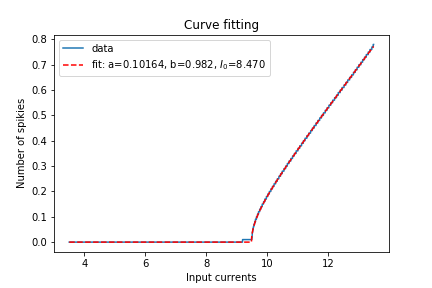
\includegraphics[width = 0.7 \textwidth]{../papers_studies/figs/Rotational/spikies_num_vs_input_fitted_curve_g50_input_3.5_13.5.png}
	\caption{تعداد تیزه برحسب جریان تصادفی برای سامانه‌ای با ده هزار نورون و ضریب تاثیر $g=50$}
	\label{fig:spikes_num_vs_background_current}
\end{figure}


تعداد تیزه‌های کل شبکه رابطه‌ی مستقیمی با جریان خارجی جاری در شبکه دارد. می‌توانیم با محاسبات تحلیلی نیز به شکل به دست آمده از شبیه‌سازی عددی نزدیک شویم:

\begin{align}
	\begin{cases}
		I_{in} &= -g \int_{a_{min}}^{a_{max}} p(a) f(a + I_{in}) da, \\
		f(a) &= \frac{\sqrt{a^2 - 1}}{2\pi}.
	\end{cases}
	\label{eq:analytical_input_current}
\end{align}

در رابطه \ref{eq:analytical_input_current} ، $f(a)$ تابع فعالیت (تعداد تیزه بر ثانیه) تک نورون بر حسب جریان کل ورودی آن است. همچنین $I_{in}$ مجموع همه‌ی جریان‌های داخلی جاری در شبکه است.\\

حل این رابطه کمی دشوار است زیرا جریان کل را بر حسب خودش محاسبه کرده است. اما از آنجایی که در انتگرال‌ده تنها یک جابجایی ثابت رخداده است؛ صورت کلی پاسخ انتگرال تغییر نمی‌کند و به صورت زیر به دست خواهد آمد.
\begin{align}
	I_{in} = \frac{-g}{2} \bigg(-a \sqrt{-1 + a^2} + log(a + \sqrt{-1 + a^2}\bigg) \Big|_{a_{min} + I_{in}}^{a_{max} + I_{in}} .
\end{align}
بی‌تردید حل معادلهٔ اخیر آشکار کننده‌ی مقدار
$I_{in}$
خواهد بود البته به شرط قابلیت حل!\\

ظاهرا گرفتن انتگرال و حل دقیق معادله کار ساده‌ای نیست. یک پیشنهاد راه حل عددی برای این مسئله این است که تابع فعالیت را با رابطه‌ی پارامتری زیر هم‌خوانی بدهیم و مقدار 
$I_0$
را پیدا کنیم،

\begin{align}
	f(I) = a \frac{\sqrt{[b(I - I_0 )]^2 - 1}}{2\pi} .
\end{align}
به عنوان مثال برای شکل
\ref{fig:spikes_num_vs_background_current}
مقدار جریان داخلی در حدود 
$8.47$
به دست آمده است.\\

هر چند این روش مقدار جریان داخلی را نسبتا خوب تخمین می‌زند اما اجازه بدهید همچنان به عنوان یک راه‌حل 
\emph{
سرانگشتی
}
یاد کنیم. زیرا شامل توصیف محدودی است از هر آن چه که در سامانه رخ می‌دهد.

\زیرقسمت{پهن‌کردن قالی صفحه‌ی فاز}
در قسمت‌های پیشین تنها به مطالعهٔ تاثیر ضریب اتصال در تغییرفاز پرداختیم و زمان تاخیر را تنها در $t_d = 0.1$ خلاصه کردیم. حال اجازه دهید تا به تاخیر نیز اجازه‌ی تغییر دهیم. در ادامه‌ی این قسمت از نوشتارمان، به فرش‌کردن صفحه‌ی فاز خود خواهیم پرداخت. امید است که چهره‌ی تمام نمای سامانه‌ بر صورت این قالی نقش بندد.\\


\زیرزیرقسمت{قالی انحراف از معیار میدان}
در شکل \ref{fig:rot_g_d_phase_space} مشاهده می‌کنیم که شدت هم‌گامی در هر کدام از هنگردهای سامانه چقدر است. بنظر می‌رسد که با افزایش زمان تاخیر و ضریب تاثیر همگامی قدرت پیدا می‌کند و هر دو در ظهور این رفتار شریک هستند. دقیقا به سان قالی مدل انباشت‌وشلیک که هم‌گامی با دو مشخصه‌ی یاد شده، رابطه‌ای مستقیم داشت.\\

\زیرقسمت{امکانی برای توصیف تحلیلی؟}
همان‌طور که پیشتر گفتیم برونل در مقاله‌ی خود 
\cite{brunel2000dynamics}
راه‌حلی تحلیلی برای توصیف گذر فاز در مدل انباشت‌وشلیک ارائه کرده است. شاید بتوان به پیروی از او راه‌حلی برای مدل چرخنده ارائه کرد اما حضور جمله‌ی غیرخطی
$- \cos\theta$
حل مسئله‌ی چرخنده‌ را بسیار دشوار کرده است. تا تاریخ نوشتن این بند، راه‌حلی تحلیلی با برداشت از برونل برای توصیف گذرفاز آن نیافته‌ایم. حال که با ابعاد دشوار مسئله روبرو شده‌ایم؛ اجازه دهید که زمین بازی خود را عوض کنیم.\\

یک قدم با احتمال شکست بالا برمی‌داریم و جمله‌ی غیرخطی درون برهم‌کنش را به کلی حذف می‌کنیم. اگر کیفیت گذارفاز هم‌چنان پابرجا بود؛ مسئله‌ی تحلیلی ما بسیار ساده و هموار می‌شود. اگر این اتفاق نیافتد جمله‌ی کسینوسی را باز می‌گردانیم و کلید حل مسئله را فقط در آن جستجو می‌کنیم.\\

اجازه بدهید تا از این پس مدل معرفی شده را با نام 
\emph{
«شبکه‌ نورون‌های ساده»
}
صدا کنیم. در بخش بعد به شبیه‌سازی این مدل می‌پردازیم. باشد که گذرفاز هم‌چنان اتفاق افتد.

%\فصل{شبکه‌ نورون‌های ساده}
	\label{chap:simple_non_repulsive}
حل مسئله‌ی مدل چرخنده‌ بسیار دشوار است و تا تاریخ نوشتن این بند، راه‌حلی تحلیلی برای توصیف گذرفاز آن نیافته‌ایم. علت این موضوع هم حضور جمله‌ی غیرخطی $- cos(\theta)$ در جمله‌ی برهم‌کنش‌های آن‌هاست. حال که با ابعاد دشوار مسئله روبرو شده‌ایم؛ اجازه دهید که زمین بازی خود را عوض کنیم.\\
می‌پرسیم که آیا کیفیت گذرفاز از ناهم‌گامی به هم‌گامی به این جمله وابسته است؟ بی‌تردید پاسخ این سوال را نخواهیم فهمید؛ مگر آن که شبکه‌ی جدیدی مطابق درخواست خود ابداع و شبیه‌سازی کنیم. این مدل را در جعبه‌ی زیر تعریف کرده‌ایم. عملا تنها کاری که کرده‌ایم حذف جمله‌ی غیر خطی است. به این ترتیب مدل بسیار ساده شده است.

\begin{tcolorbox}
	\begin{equation}
		\begin{cases}
			\dot{\theta_i}=I_i  - g E, \hspace{2ex}  \theta_i \leq \pi \\
			\dot{E} = M - \alpha E\\
			\dot{M} = -  \alpha M + \frac{ \alpha^{2} }{N} \sum_{n|tـn<t} \delta(t - t_n - t_d)
		\end{cases}
	\end{equation}
	\begin{enumerate}[-]
		\item $\theta_i$:
		مشخص کننده‌ی فاز هر نورون. این فاز میان دو لبه در حال حیات است. کوچکترین کران بالای آن همان حالت آستانه در $\pi$ است و بزرگترین کران پایین آن نگه‌دارنده‌ای است که از ریزش نورون‌ها جلوگیری می‌کند.
		\item $E$:
		میدانی است که شدت فعالیت شبکه را نشان می‌دهد.
		\item $M$:
		یک پارامتر فرعی که در حل معادله دیفرانسیل مرتبه دوم به دو معادلهٔ تحول مرتبه اول ما را یاری کرده است.
	\end{enumerate}
\end{tcolorbox}

همچنین دقت کنیم که اگر چه این مدل کاهش یافته‌ای از مدل چرخنده است اما در صورت کاستن مدل انباشت‌وشلیک هم به همین جملات برهم‌کنشی می‌رسیدیم. تنها تفاوت در آن می‌شد که فاصله‌ی بین حالت تیزه ($\pi$) و بازنشانی (صفر) در حالت ابداعی $\pi$ برابر مدل کاسته‌شده‌ی انباشت‌وشلیک می‌شد.

\قسمت{شبیه‌سازی}
برای مدل توصیف شده‌ی بالا شبیه‌سازی خود را با تنظیمات زیر به اجرا گذاشتیم. 
\begin{tcolorbox}[colback=green!5!white,colframe=green!75!black]
	\begin{enumerate}[*]
		\item
		$\alpha = 20\, s^{-1}$
		\item
		جریان‌های تصادفی خارجی نورون‌ها از اعضای بازه‌ی $(9.5,13.5)$ انتخاب می‌شوند.
		\item
		$N = 10000$
		\item
		$t_d = 0.1\, s$ 
	\end{enumerate}
\end{tcolorbox}

\قسمت{نتایج}
\زیرقسمت{در جستجوی تغییرفاز}
قابل توجه است که کیفیت تغییرفاز با حذف جمله‌ی ذکر شده تغییر نکرد و تنها مکان و ارتفاع انحراف از معیار جریان داخلی است که دست خور تغییر شده است - شکل \ref{fig:sigma_non_repulsive}. نکته‌ی جالب‌تر اینجاست که صفحه‌ی فاز هم تقریبا همان رنگ‌آمیزی را دارد که در برای نورون‌های دیگر دیدیم. به جهت اهمیت نکات پیشین اجازه بدهید ملاحظات را یک بار دیگر اینجا آوریم:\\

\begin{enumerate}[1.]
	\item 
	به نظر می‌رسد که با افزایش زمان تاخیر و ضریب تاثیر همگامی قدرت پیدا می‌کند
	\item 
	برای ضریب‌تاثیر یک گذرفاز کاملا ناگهانی و برای تاخیر زمانی که گذرفازی ملایم!
	\item 
	اگر چه تاخیر در جابجایی ضریب‌تاثیر بحرانی تغییری ایجاد نکرده است اما هم‌گامی را قدرت می‌بخشد.
	\item
	اگر ضریب‌تاثیر را بسیار بزرگ کنیم و فاصله‌ی زیادی از ضریب‌تاثیر بحرانی بگیریم؛ شدت هم‌گامی ضعیف می‌شود. این نکته می‌تواند به علت رشد جمعیت نورون‌های خاموش باشد که از تیزه‌زدن محروم می‌شوند و نمی‌توانند خیزهای بلندی را به جریان داخلی القا کنند.
\end{enumerate}



\begin{figure}
	\begin{subfigure}{0.5\textwidth}
		\centering
		\includegraphics[width = \textwidth]{../scripts/all_neurons_model_in_one_place/Non_repulsive_rotational_ensembles/N10000_T100_I9.5_13.5_v1.0/sigma_g_0_130.png}
		\caption{پهنای جریان یک سامانه ساده با ده هزار نورون}
		\label{fig:sigma_non_repulsive}
	\end{subfigure}
	\hfill
	\begin{subfigure}{0.5\textwidth}
		\includegraphics[width = \textwidth]{../scripts/all_neurons_model_in_one_place/Non_repulsive_rotational_ensembles/N10000_T100_I9.5_13.5_v1.0/sigma_phase_space_contour_alpha20.png}
		\caption{
			صفحه‌ی فاز شبکه نورون‌های ساده: پیوست:
			\ref{appendix:phase_samplingـrotational}
		}
		\label{fig:if_g_d_phase_space_Non_repulsive}
	\end{subfigure}
\end{figure}

\زیرقسمت*{تاملی برای گام بعدی}
به نظر می‌آید قدمی که به سمت حذف جمله‌ی غیرخطی داشتیم کاملا مفید بود. زیرا مدل را با حفظ خاصیت گذر فاز، ساده‌تر کرد.  به راستی چه اتفاقی دارد در پس پرده می‌افتد؟ سامانه‌ی هم‌گام با ناهم‌گام چه تفاوت‌هایی دارد؟ پاسخ به این سوال‌ها با مطالعهٔ اعداد خروجی کاری دشوار است زیرا همواره همراه با حدس و گمان ذهنی است. بیاید قدم بعدی را به سمت «تصویرسازی» برداریم.


\فصل{تلاش برای توصیف}

از آنجا که شبیه‌سازی این سامانه شامل تعریف فرآیندهای متفاوتی بود؛ بدیهی است که نوشتن معادله‌ی تحلیلی برای توصیف کامل آن آسان نباشد. اما در این بخش تلاش می‌کنیم که با کنار هم قرار دادن معادلات اصلی چارچوب مسئله‌ی خود را مشخص کنیم.\\
هر نورون که از حالت $\theta = \pi$ عبور می‌کند [تیزه می‌زند] باعث می‌شود تا سهمی از جریان با کیفیت $p(t):= \alpha^2 t \cdot exp(-\alpha t)$ به جریان درونی کل سامانه $E(t)$ اضافه شود.
\begin{equation}
	E(t) = \frac{1}{N}\int_{0}^{\infty} \int J_a (\pi,t-d-u) da \cdot \alpha^2 u\, e^{-\alpha u} du
\end{equation}

اما جریان برای هر نورون با ورودی $a$ به طریق زیر است:
\begin{equation}
	J_a (\theta, t) = n_a(\theta,t) \cdot \dot \theta_a
\end{equation}
این رفتار به خوبی نشان می‌دهد جریان فقط در ناحیه‌ی $\theta \leq \pi$ وجود دارد. زیرا ورود نورون به ناحیه‌ی مثبت‌تر را ممنوع کرده‌ایم.  بی‌تردید برای فهمیدن چگونگی تغییر جریان در ناحیه‌های میانی باید از معادله‌ی پخش استفاده کنیم.
\begin{align}
	\frac{\partial n_a}{\partial t} &= - \frac{\partial J_a}{\partial \theta}\\
	&= - \frac{\partial n_a}{\partial \theta} \cdot \dot \theta_a
\end{align}
\زیرقسمت{حل معادله‌ی شبکه‌ی ساده}
اجازه بدهید تا اولین تلاش خود را از ساده‌ترین نوع شبکه‌ها شروع کنیم. شبکه‌ای که به جز جریان داخلی و جریان تصادفی اولیه ورودی دیگری ندارد. پس خواهیم داشت:
\begin{align}
	\begin{cases}
		E(t) = \frac{1}{N} \int_{0}^{\infty} \int n_a(\pi,t-d-u) \cdot \big[ a - g E(t-d-u) \big] da \cdot \alpha^2 u\, e^{-\alpha u} du \\
		\frac{\partial n_a}{\partial t} = - \frac{\partial n_a}{\partial \theta} \cdot (a - g E(t) )
	\end{cases}
	\label{eq:simple_network}
\end{align}
چند پیشنهاد می‌شود برای ادامه‌ی راه‌حل داشت. (درون یک جعبه قرار گیرد با این عنوان که پیشنهادات من چه بود و استاد چه گفت.)
\begin{enumerate}[1.]
	\item
	از آنجا که میدان به گونه‌ای متناوب عمل می‌کند؛ یک پیشنهاد خوب می‌تواند آن باشد که بسط فوریه‌ی آن را بنویسیم.
	\begin{equation}
		E(t) = \sum c_i \cdot cos(\omega_i t)
	\end{equation}
	که اگر ثابت کنیم $c_1$ از بقیه ضرایب بزرگتر است؛ مساله‌ی ما حل می‌شود.
	\item
	دشواری مساله از در هم تنیدگی معادلات برآمده است. اگر به تقریب در معادله‌ی پخش میدان را یک نوفه درنظر بگیریم و پاسخ را در معادله‌ی اول قرار دهیم.
	\item
	انتگرال اول را به صورت بازگشتی در خودش جاگذاری کنیم.
	\item
	مسئله را در حالت آماری بررسی کنیم و حالت پایستار آن را پیدا کنیم و  بپرسیم در چه حالتی است که حالت پایستار داریم.
\end{enumerate}



\زیرزیرقسمت{روش بازگشتی}
نکته‌ای که برای ما حل معادلات را دشوار می‌کند تبعیت $E$ از خودش است. بگذارید به شیوه‌ای که خود معادله درخواست دارد عمل کنیم. یعنی $E$ را مجددا در سمت راست معادله جاگذاری کنیم. برای راحت‌تر شدن محاسبات ابتدا دو متغیر کمکی زیر را تعریف می‌کنیم:
% abbrivations for calculation of this section
\newcommand{\J}[1]{\mathcal{J}(\pi,#1)}
\newcommand{\N}[1]{\mathcal{N}(\pi, #1)}
\newcommand{\Pexp}[1]{\mathcal{P}(u_{#1})}

\newcommand{\A}[1]{\mathcal{A}(#1)}

%\newcommand{\impact}[1]{u_{#1}\, e^{-\alpha u_{#1}}}
%
\begin{align}
	\J{t-d-u} &\equiv \int n_a(\pi,t-d-u) a \cdot da\\
	\N{t-d-u} &\equiv \int n_a(\pi,t-d-u) \cdot da\\
	\Pexp{} &\equiv \alpha^2 u\, e^{-\alpha u}
\end{align}
عبارت $\J{}$ به معنای جمع جریان تصادفی نورون‌هایی است که در زمان u در آستانه قرار دارند. همچنین عبارت $\N{}$ به معنای تعداد همین نورون‌هاست.\\
حال با نمادهای بالا شروع به بازنویسی جملات پیشین می‌کنیم:
\begin{align}
	E(t) &= \frac{1}{N} \int_{0}^{\infty} \J{t-d-u_1} \cdot \Pexp{1} du_1  - \frac{g}{N}\int_{0}^{\infty} \N{t-d-u_1} \cdot \Pexp{1} E(t-d-u_1)  du_1
\end{align}
حال جمله‌ی اول را نیز با عبارت دیگری خلاصه‌سازی می‌کنیم:

\begin{equation}
	\A{t} \equiv \frac{1}{N}\int_{0}^{\infty} \J{t-d-u_1} \cdot \Pexp{1} du_1
\end{equation}
در خصوص جمله‌ی دوم نیز مشابها عبارت مربوط به $E$ را در آن جاگذاری می‌کنیم.
\begin{align}
	E(t - d - u_1) &= \frac{1}{N} \int_{0}^{\infty} \J{t-2d-u_1-u_2} \cdot \Pexp{2} du_2\\
	&- \frac{g}{N}\int_{0}^{\infty} \N{t-2d-u_1-u_2} \cdot \Pexp{2} E(t-2d-u_1-u_2)  du_2
\end{align}

این عبارت جمع تعداد همه‌ی تیزه‌هایی است که تا گام $t-d$ زده شده‌اند و درنتیجه جمله‌ای انباشتی است. پس خواهیم داشت:
\newgeometry{top=5mm, bottom=5mm}
%your text here  
\begin{landscape}
	\begin{align}
		E(t) &= \A{t-d} - g\int_{0}^{\infty} \N{t-d-u_1} \cdot \Pexp{1} E(t-d-u_1) du_1\\
		&= \A{t-d} - g\int_{0}^{\infty} \N{t-d-u_1} \cdot \Pexp{1} \cdot \big[ \A{t-2d-u_1} - g\int_{0}^{\infty} \N{t-d- u_1-u_2} \cdot \Pexp{2} E(t-2d-u_1-u_2) du_2 \big] du_1\\
		&= \A{t-d} - g\int_{0}^{\infty} \N{t-d-u_1} \cdot \Pexp{1} \cdot \A{t-2d-u_1} du_1\\ 
		&\hspace{1 cm}+ g^2 \int_{0}^{\infty} \N{t-d-u_1} \cdot \Pexp{1}\int_{0}^{\infty} \N{t-2d-u_1-u_2} \cdot \Pexp{2} E(t-2d-u_1-u_2) du_2 du_1\\
		&= \A{t-d} - g\int_{0}^{\infty} \N{t-d-u_1} \cdot \Pexp{1} \cdot \A{t-2d-u_1} du_1\\ 
		&\hspace{1 cm}+ g^2 \int_{0}^{\infty} \N{t-d-u_1} \cdot \Pexp{1}\int_{0}^{\infty} \N{t-2d-u_1-u_2} \cdot \Pexp{2} \A{t-3d-u_1-u_2} du_2 du_1\\
		&\hspace{1 cm}- g^3 \int_{0}^{\infty} \N{t-d-u_1} \cdot \Pexp{1}\int_{0}^{\infty} \N{t-2d-u_1-u_2} \cdot \Pexp{2} \int_{0}^{\infty} \N{t-3d-u_1-u_2-u_3} \cdot \Pexp{3} E(t-3d-u_1-u_2-u_3) du_3 du_2 du_1
	\end{align}
\end{landscape}

\restoregeometry 

حال اگر عمر این سامانه کراندار باشد؛ تعداد جملات بالا محدود می‌شوند. پس اگر سامانه پیش از یک زمانی کاملا خاموش بوده باشد$E = 0$؛ آنگاه می‌توان میدان کنونی را بر اساس جملات ضربی بین شدت جریان و تعداد نورون‌های تیزه زده پیدا کرد.


\زیرزیرقسمت{روش اختلال}
به نمودار \ref{fig:sigma_rotational} دقت کنید. در زمانی که تعداد نورون‌ها بی‌نهایت باشد؛ در فاز ناهم‌گام انحراف معیار میدان صفر خواهد شد. این به این معنی است که جریان در زمان ثابت خواهد ماند. پس بگذارید با علم بر این موضوع یک جواب معادله‌ی \ref{eq:simple_network} را در حالت حدی میدان ثابت $E_0$ معرفی کنیم.\\
با فرض ثابت بودن میدان، اندازه‌ی آن را محاسبه می‌کنیم. سپس مجدد به معادلات برمی‌گردیم و می‌پرسیم که در صورت جمع با یک جمله‌ی اختلالی کوچک این انحراف رشد خواهد کرد یا خیر. به عبارت دیگر آیا این جواب جاذب است.\\
\begin{align}
	\begin{cases}
		E_0 = \frac{1}{N}\int_{- \infty}^{t - d} \int n_a(\pi,u) \cdot \big[ a - g E_0 \big] da \cdot \alpha^2 u\, e^{-\alpha u} du \\
		\frac{\partial n_a}{\partial t} = - \frac{\partial n_a}{\partial \theta} \cdot (a - g E_0 )
	\end{cases}
\end{align}

یک راه خوب برای پیشبرد سطر اول معادلات آن است که از دو طرف آهنگ تغییرشان با زمان را بپرسیم. از آنجا که سمت چپ معادله ثابت است؛ سمت راست هم باید جوابی مشابه را حکایت کند.\\
\begin{equation}
	0 = \frac{dE_0}{dt} = \frac{\alpha^2 (t-d) e^{-\alpha (t-d)}}{N} \cdot [ - gE_0 \cdot \int n_a(\pi,t-d) da + \int n_a(\pi,t-d)\cdot a\,da ]
\end{equation}
مشخص است که کدام جمله از جملات ضربی بالا صفر است. پس برای $E_0$ خواهیم داشت:
\begin{equation}
	E_0 = \frac{1}{g}\cdot \frac{\int n_a(\pi,t-d)\cdot a\,da}{\int n_a(\pi,t-d) da }
\end{equation}

حال برای ادامه‌ی فرآیند نیاز داریم تا عبارت حاکم بر 
$n_a(\pi,t-d)$
را بدست آوریم. جواب پیشنهادی ما برای سطر دوم معادلات از جنس تابع دلتاست:
\begin{align}
	n_a(\theta,t) &= \delta(\theta - \theta_a(t)) \\
	&= \delta(\theta + \theta_0 - (a - g E_0)t + 2 \floor{K^{(t)}_a}\pi )\\
	&= \delta( \theta - (a - g E_0)t + 2 \floor{K^{(t)}_a} \pi + \theta_0  )\\
	\Rightarrow n_a(\pi,t) &= \delta(  (2\floor{K^{(t)}_a} + 1)\pi - (a - g E_0)t + \theta_0   )\\
\end{align}
که در این معادلات 
$K^{(t)}_a$
کسری است که تعداد دور هر نورون را از آغاز تا کنون روایت می‌کند و ما مجبور به عقب کشیدن 
$2\pi$
فاز کامل پس از تیزه زدن آن به تعداد 
$\floor{K^{(t)}_a}$
شده‌ایم.
\footnote{دقت کنیم که معادله‌ی ذکر شده برای نورون‌هایی درست است که 
	$(a - g E_0) > 0 $
}
قابل محاسبه است که عبارت کامل آن به صورت زیر است.
\begin{equation}
	K^{(t)}_a = \frac{(a - gE_0)t + \pi + \theta_0}{2\pi}
\end{equation}

برای محاسبه‌ی انتگرال‌هایی که شامل این دلتای دیراک هستند؛ لازم است تا صفر‌های آرگومان آن را محاسبه کنیم.
\begin{align}
	\big( 2 \floor{\frac{(a - gE_0)t + \pi + \theta_0}{2\pi}} + 1 \big)\pi - (a - g E_0)t + \theta_0 &= 0\\
	2\pi \times \bigg( \floor{\frac{(a - gE_0)t + \pi + \theta_0}{2\pi}}  - \frac{(a - gE_0)t + \pi + \theta_0}{2\pi} \bigg) &= 0\\
	2\pi \times \bigg( \floor{K^{(t)}_a} - K^{(t)}_a \bigg) &= 0  \label{eq:neuron_pattern_simple_model}
\end{align}
این رابطه کاملا یک تابع تناوبی را توصیف می‌کند. یک تابع مقطع که در مکانی که آرگومان آن صحیح می‌شود؛ مقدار صفر به خود می‌گیرد. پس روشن است که توقع داشته باشیم. تعداد صفرهای این معادله به اندازه‌ی تعداد تناوبی است که در هر زمان در بازه‌ی جریان‌های داده شده دارد.
\begin{align}
	\Delta K^{(t)}_a  &= 1\\
	\Delta K^{(t)}_a &= \frac{t}{2\pi}\Delta a\\
	\Delta a &= \frac{2\pi}{t}
\end{align}
این دوره‌ی تناوب با افزایش زمان کوچکتر می‌شود. اگر تعداد نورون‌ها را به صورتی ترمودینامیکی بزرگ بگیریم؛ آنگاه به ازای هر دوره‌ی تناوب یک نورون حتما هست که روی محور آستانه قرار گرفته است.\\
حال که دوره‌ی تناوب 
$\Delta a$
را بدست آوردیم؛ می‌دانیم که ریشه‌های رابطه‌ی 
\ref{eq:neuron_pattern_simple_model}
چه زمانی رخ می‌دهند. فرض کنیم که اولین صفر در جریانی مثل
$a_m$
رخ می‌دهد. توجه کنید حتما اندازه‌ی این جریان به گونه‌ای است که نورون را به صورت فعال نگه دارد. پس باید حتما
$(a_m - g E_0) > 0 $
باشد.
حال می‌توانیم انتگرال‌های مورد نظر خود را این چنین بسط دهیم.

\begin{align}
	\int n_a(\pi,t-d)a\,da &= \int \delta \bigg( 2\pi ( \floor{K^{(t)}_a} - K^{(t)}_a) \bigg) a\,da\\
	&= \frac{1}{2\pi} \cdot \sum_{K^{(t)}_a \in Z} a_i \\
	&= \frac{1}{2\pi} \cdot \sum^{M}_{m=0} a_m + m \cdot \Delta a\\
	&= \frac{M+1}{2\pi} \cdot ( \frac{a_m +a_{max} }{2} )\\
\end{align}
و از طرفی:
\begin{align}
	\int n_a(\pi,t-d)\,da &= \int \delta \bigg( 2\pi ( \floor{K^{(t)}_a} - K^{(t)}_a) \bigg) a\,da\\
	&= \frac{1}{2\pi} \cdot \sum_{K^{(t)}_a \in Z} 1 \\
	&= \frac{1}{2\pi} \cdot \sum^{M}_{m=0}  1\\
	&= \frac{M+1}{2\pi}
\end{align}
حال اگر به محاسبه‌ی میدان ثابت خود برگردیم و تکه‌های پازل را کنار هم بگذاریم؛ خواهیم داشت:
\begin{align}
	E_0 &= \frac{1}{g}\cdot \frac{\int n_a(\pi,t-d)\cdot a\,da}{\int n_a(\pi,t-d) da } \\
	&= \frac{1}{g}\cdot \frac{ \frac{M+1}{2\pi} \cdot ( \frac{a_m +a_{max} }{2} ) }{ \frac{M+1}{2\pi} } \\
	&= \frac{1}{g} ( \frac{a_m +a_{max} }{2} )
\end{align}
این میدان معادل است با جریان میانگین بین نورون‌هایی که آن‌ها را روشن خطاب کرده بودیم. این نتیجه صحیح نیست زیرا اگر میدان در میانه‌ی این جریان‌ها قرار گیرد؛ آنگاه نورون‌های با جریان پایین‌دست 
$a < \frac{1}{g} ( \frac{a_m +a_{max} }{2} ) $
را خاموش خواهد کرد و اصلا روشن نخواهند ماند.

\زیرزیرقسمت{روش آماری}
در این روش فرض می‌کنیم که برای هر جریان تصادفی اولیه، نورون‌های زیادی را به اختیار گرفته‌ایم. در حالت پایا  ، در یک حالت خاص تغییری در چگالی جمعیت مشاهده نمی‌شود پس در معادله‌ی
\ref{eq:simple_network}
خواهیم داشت:
\begin{equation}
	\frac{\partial n_a}{\partial t} = 0
\end{equation}
همچنین در حالت پایا که در واقع از نگاه ما حالت ناهم‌گام است؛ جریان بین نورون‌ها - که کمیتی بزرگ مقیاس است -  در زمان تغییری نمی‌کند. پس به این ترتیب:

\begin{align}
	\begin{cases}
		\frac{\partial n_a}{\partial t} = - \frac{\partial J_{a}(t)}{\partial \theta} = 0\\
		J_{a}(\theta, t) = n_a(\theta,t) \cdot [ a - g E ]\\
	\end{cases}
	\Rightarrow J_{a}(\theta, t) = J_{a}(t)\\
	\Rightarrow n_{a}(\theta, t) = n_{a}\\
\end{align}

پس توزیع جمعیت نورون‌‌ها مستقل از زمان و حالت آن‌ها خواهد شد. اگر توزیع را در ابتدا یکنواخت میان جریان‌های مختلف توزیع کرده باشیم؛ برای همه‌ی زمان‌ها و حالت‌ها داریم:
\begin{equation}
	n = \frac{N}{2 \pi (a_{Max} - a_{min}) }
\end{equation}


برای جریان بین نورون‌ها هم خواهیم داشت:
\begin{align}
	E &= \frac{1}{N} \int_{- \infty}^{t - d} \int n \cdot \big[ a - g E \big] da \cdot \alpha^2 u\, e^{-\alpha u} du\\
	&=  \int \frac{n}{N} \cdot \big[ a - g E \big] da \label{eq:e_sum_simple}
\end{align}
دقت کنیم که انتگرال رابطه‌ی \ref{eq:e_sum_simple} روی  نورون‌هایی است که مستعد تیزه زدن هستند.
\footnote{
	$(a - g E) > 0 $
}

اولین جریانی که نورون را مستعد تیزه زدن می‌کند $a_*$ نام‌گذاری می‌کنیم. وقتی جریان مهاری حاصل از تیزه زدن‌ها کوچک است؛ همه‌ی نورون‌ها فعال هستند و در نتیجه‌ 
$a_* = a_{min}$
می‌شود. اما در حالتی که جریان مهاری زیاد می‌شود؛ این مقدار از کمترین جریان تصادفی اولیه سامانه بزرگتر می‌شود. محاسبات را ادامه می‌دهیم:
\begin{align}
	E &=  \int \frac{n}{N} \cdot \big[ a - g E \big] da \\
	&= \frac{n}{N} \cdot \big[ \frac{a^2_{Max} - {a_*}^2}{2} - g E (a_{Max} - a_*) \big] \\
	\Rightarrow E &= n \cdot \big[ \frac{a^2_{Max} - {a_*}^2}{2}  \big] / \big[ N + g n (a_{Max} - a_*)\big]
	\label{}
\end{align}
شاید بنظر این یک معادله‌ی درجه یک ساده باشد که میدان را گزارش می‌کند اما در واقع خود $a^*$ هم به میدان وابسته است و باید وابستگی آن را لحاظ کنیم. به تقریب:
$a^{*} = gE$
با اضافه کردن این معادله و حل معمول یک معادله‌ی درجه‌ی دو برای میدان صراحتا خواهیم داشت:
\begin{align}
	E =  \big( \frac{a_{Max}}{g} + \frac{N}{n g^2}  \big) \pm \big[ \big( \frac{N}{n g^2} + \frac{a_{Max}}{g} \big)^2 - \frac{{a_{Max}}^2}{g^2} \big]^{\frac{1}{2}}
\end{align}
نتیجه می‌دهد که $a_{*}$ هم باید به صورت زیر باشد:
\begin{align}
	a_{*} &=  \big( a_{Max} + \frac{N}{n g} \big) \pm \big[ \big( \frac{N}{n g} + a_{Max} \big)^2 - {a_{Max}}^2 \big]^{\frac{1}{2}}\\
	&=  \big( a_{Max} + \frac{N}{n g} \big) \pm \big[  \frac{N^2}{n^2 g^2} + \frac{2a_{Max}N}{ng}  \big]^{\frac{1}{2}}
\end{align}
اجازه بدهید علامت مثبت را کنار بگذاریم زیرا مقدار $a_{*}$ را خارج بازه‌ی جریان‌های سامانه گزارش می‌کند. پس هم برای میدان و هم جریان $a_{*}$ خواهیم داشت:
\begin{align}
	\begin{cases}
		a_{*} =  \big( a_{Max} + \frac{N}{n g} \big) - \big[  \frac{N^2}{n^2 g^2} + \frac{2a_{Max}}{ng}  \big]^{\frac{1}{2}}\\
		E =  \big( \frac{a_{Max}}{g} + \frac{N}{n g^2} \big) - \big[ \frac{N^2}{n^2 g^4} + \frac{2Na_{Max}}{ng^3}  \big]^{\frac{1}{2}}\\
	\end{cases}
\end{align}

حال اگر نتایج بدست آمده را با داده‌های شبیه‌سازی تطبیق دهیم؛ خواهیم دید که تطابق خوبی با یک دیگر دارند.

\begin{figure}
	\centering
	\begin{subfigure}[b]{0.5\textwidth}
		\centering
		\includegraphics[width=\textwidth]{../scripts/all_neurons_model_in_one_place/Non_repulsive_rotational_ensembles/N10000_T100_I9.5_13.5_v1.0/field_zeroth_order_asterix_g_0.1_130.png}
		\caption{نسخه‌ای که کمینه‌ی جریان را از حل محاسبات درنظر می‌گیرد}
		\label{fig:e_zeroth_not_all_gifted}
	\end{subfigure}
	\hfill
	\begin{subfigure}[b]{0.5\textwidth}
		\centering
		\includegraphics[width=\textwidth]{../scripts/all_neurons_model_in_one_place/Non_repulsive_rotational_ensembles/N10000_T100_I9.5_13.5_v1.0/field_zeroth_order_simple_g_0.1_130.png}
		\caption{نسخه‌ای که همه‌ی نورون‌ها را فعال تصور می‌کند.}
		\label{fig:e_zeroth_all_gifted}
	\end{subfigure}
	\hfill
	\begin{subfigure}[b]{0.5\textwidth}
		\centering
		\includegraphics[width=\textwidth]{../scripts/all_neurons_model_in_one_place/Non_repulsive_rotational_ensembles/N10000_T100_I9.5_13.5_v1.0/field_zeroth_order_developed_g_0.1_130.png}
		\caption{نسخه ساخته شده از اتصال دوتای دیگر}
		\label{fig:e_zeroth_developed}
	\end{subfigure}
	\caption{تطابق جریان پایای بدست آمده از حل عددی و تحلیلی}
	\label{fig:three graphs}
\end{figure}

در ضریب تاثیرهای بسیار بزرگ داریم:
\begin{align}
	E \cong & \frac{a_{Max}}{g} + \frac{N}{ng^2} - (\frac{2N a_{Max}}{n g^3})^{\frac{1}{2}} \big[ 1 + \frac{N}{2nga_{Max}} \big]^{\frac{1}{2}}\\
	=& \frac{a_{Max}}{g} + \frac{N}{ng^2} - (\frac{2 N a_{Max}}{n g^3})^{\frac{1}{2}} \big[ 1 + \frac{N}{4nga_{Max}} \big]\\
	=& \frac{a_{Max}}{g} - (\frac{2 N a_{Max}}{n g^3})^{\frac{1}{2}} + \frac{N}{ng^2}  - (\frac{N}{2n})^{\frac{3}{2}}  \cdot \frac{1}{ {a^{\frac{1}{2}}_{Max} g^{\frac{5}{2}}}}
\end{align}


\زیرزیرقسمت{حل اختلالی میدان}
همان طور که مشخص است؛ حل دقیق میدان بسیار کار دشواری است اما می‌توان از طریق ترفندهای اختلالی به جواب آن نزدیک شد. یکی از روش‌های معمول حل زنجیری و تودرتوی دستگاه معادلات است. \\
به این ترتیب که ابتدا از معادله  پاسخ حالت پایا (مرتبه‌ی صفرم) را در معادله‌ی پخش جاگذاری می‌کنیم تا توزیع آماری وابسته به زمان نورون‌ها بدست آید. سپس مجددا از توزیع بدست آمده؛ میدان مرتبه‌ی اول را که وابسته به زمان است؛ محاسبه می‌کنیم.\\
از آنجا که توزیع سامانه‌ رفتاری دوره‌ای به طول $2\pi$ دارد؛ می‌توانیم آن را به صورت زیر بسط دهیم:
\begin{align}
	\rho(\theta, a, t) = \rho_0 + \sum_k A_k(t) e^{ik\theta}, \quad k \in \mathcal{Z}
\end{align}

\begin{align}
	\frac{\partial \rho}{\partial t} &= \sum \dot A_k e^{ik\theta}\\
	\frac{\partial \rho}{\partial \theta} &= \sum A_k \cdot ik \cdot e^{ik\theta}\\
\end{align}
حال آن را در معادله‌ی پخش قرار می‌دهیم تا بتوانیم معادله‌ی حاکم بر ضرایب را محاسبه کنیم.
\begin{align}
	\sum \dot A_k e^{ik\theta} &= - \sum A_k \cdot ik(a - gE(t)) \cdot e^{ik\theta}\\
	\Rightarrow \dot A_k &= - A_k \cdot ik(a - gE(t))
\end{align}
در تقریب مرتبه‌ی اول برای توزیع داریم:
\begin{align}
	\dot A_k &= - A_k \cdot ik(a - g E_0)\\
	\Rightarrow A_k(t) &= A_k(0) e^{- ik(a-gE_0)t}\\
	\Rightarrow \rho(\theta, a, t) &= \rho_0 + \sum_k A_k(0) e^{ik\theta - ik(a - gE_0)t}
\end{align}
پس برای نورون‌های روی آستانه خواهیم داشت:
\begin{align}
	\rho(\pi, a, t) = \rho_0 + \sum_k A_k(0) e^{ik\pi - ik(a - gE_0)t}
\end{align}
حال از نتیجه‌ی بدست آمده استفاده می‌کنیم و همان طور که اشاره شد به محاسبه‌ی مرتبه‌ی بعدی میدان می‌رویم:
\begin{align}
	E(t) &= \int \int_{0}^{\infty} \rho(\pi, a, t-d-v)\cdot \dot \theta \cdot \alpha^2 ve^{-\alpha v} dv da \label{eq:perturbed_field}\\
	&= E_0\\
	&+ \int \int_{0}^{\infty} \sum_k A_k(0) e^{ik\pi - ik(a - gE_0)(t-d - v)} \cdot (a - gE_0) \alpha^2 ve^{-\alpha v} dv da \\
	&= E_0 + \sum_k \int \int_{0}^{\infty} A_k(0) e^{ik\pi - ik(a - gE_0)(t-d - v)} \cdot (a - gE_0) \alpha^2 ve^{-\alpha v} dv da
\end{align}
اجازه بدهید سهم مدهای متفاوت از میدان را به صورت جداگانه محاسبه کنیم و سپس مجددا در کنار یکدیگر قرار دهیم.
\begin{align}
	E_{k,a}(t) = -\alpha^2 A_k(0)(a - gE_0) e^{ik\pi}\int^{\infty}_{0} v e^{-[\alpha - ik(a - gE_0)]v-ik(a - gE_0)(t-d)} dv
\end{align}
با با تغییر متغیر 
$\beta \equiv \alpha - ik(a-gE_0)$
محاسبات را ادامه می‌دهیم:
\begin{align}
	&= \alpha^2 A_k(0) (a - gE_0) e^{ik\pi} e^{-ik(a-gE_0)(t-d)} \cdot \int^{\infty}_0 v e^{-\beta v}dv \\
	&= \alpha^2 A_k(0) (a - gE_0) e^{ik\pi} e^{-ik(a-gE_0)(t-d)} \cdot \frac{1}{\beta^2} \\
	&= A_k(0) (a - gE_0) e^{ik[\pi -(a-gE_0)(t-d)]} \cdot (\frac{\alpha}{\alpha-ik(a-gE_0)})^2
\end{align}
حال قدم به قدم به محاسبات پیشین خود برمی‌گردیم. ابتدا می‌پرسیم میدان همه‌ی نورون‌های با مد یکسان چه جریانی را تولید می‌کنند.
\begin{align}
	E_k(t) &= \int E_{k,a} da\\
	&= \int A_k(0) (a - gE_0) e^{ik[\pi -(a-gE_0)(t-d)]} (\frac{\alpha}{\alpha-ik(a-gE_0)})^2 da
\end{align}
با تغییر متغیر
$h \equiv a - gE_0$
تلاش می‌کنیم انتگرال را ادامه دهیم.
\begin{align}
	E_k(t) = A_k(0)e^{ik\pi} \int^{a_M - gE_0}_{0} h e^{-ikh(t-d)} (\frac{1}{1 - ikh/\alpha})^2 dh
\end{align}
نرم‌افزارهای محاسباتی همچون ابزار ولفرم به ما امکان می‌دهد تا پاسخ آن را به صورت زیر بیان کنیم:
\begin{align}
	E_k(t) = -A_k(0)\frac{\alpha^2}{k^2} e^{ik\pi} &\bigg[ \frac{ e^{-i(\xi_{(h)} + k(t-d)h)} }{\sqrt{1 + h^2 k^2/\alpha^2}} \\
	&+ e^{-\alpha(t-d)}(\alpha(t-d) + 1) Ei[(\alpha-ikh)(t-d)] \, \bigg]	\Biggr|_{0}^{a_M -gE_0}
\end{align}
به صورتی که 
$e^{-i\xi_{(h)}} = \frac{1 + ikh/\alpha}{\sqrt{1 + h^2 k^2/\alpha^2}}$
است و 
$Ei$
همان تابع انتگرال نمایی است که به صورت 
$Ei[z] = - \int^{+\infty}_{-z} e^{-t}/t dt$
نوشته می‌شود.
\begin{align}
	E_k(t) =& - A_k(0) \frac{\alpha^2}{k^2} e^{ik\pi} \bigg[ \frac{ e^{-i(\xi_{(a_M -gE_0)} + k(t-d)(a_M -gE_0))} }{\sqrt{1 + (a_M -gE_0)^2 k^2/\alpha^2}} \\
	&+ e^{-\alpha(t-d)}(\alpha(t-d) + 1) Ei[(\alpha-ik(a_M -gE_0))(t-d)] \\
	&- e^{-ik(t-d)(a_M -gE_0)} \\
	&- e^{-\alpha(t-d)}(\alpha(t-d) + 1) Ei[\alpha(t-d)] \bigg]\\
	=&- A_k(0) \frac{\alpha^2}{k^2} e^{ik\pi} \bigg[ e^{-ik(t-d)(a_M -gE_0)} \bigg( \frac{ e^{-i(\xi_{(a_M -gE_0)})} }{ \sqrt{1 + (a_M -gE_0)^2 k^2/\alpha^2} } + 1\bigg) \\
	&+ e^{-\alpha(t-d)}(\alpha(t-d) + 1)\bigg( Ei[(\alpha-ik(a_M -gE_0))(t-d)] - Ei[\alpha(t-d)] \bigg) \bigg]
\end{align}
پس یک جمله‌ی نوسانی دارد و جمله‌ای که شامل تکینگی است.\\
خبر خوب یا بد این است که این راه هم دارای ایراد است. زیرا در محاسبه‌ی مرتبه‌ی اول میدان اشتباهی رخداده است - رابطه‌ی \ref{eq:perturbed_field}.
در این رابطه باید ضرب مرتبه‌ی صفرم چگالی در مرتبه‌ی اول میدان جا مانده است. یعنی باید می‌نوشتیم:
\begin{align}
		E(t) &= \int \int_{0}^{\infty} (\rho_0 + \rho_1)(a - g(E_0 + E_1) ) \cdot \alpha^2 ve^{-\alpha v} dv da \\
		&= \int \int_{0}^{\infty} [\rho_0(a - gE_0) + \rho_1 (a - gE_0)] \cdot \alpha^2 ve^{-\alpha v} dv da \\
		&+ \int \int_{0}^{\infty} -g E_1 \rho_1 \cdot \alpha^2 ve^{-\alpha v} dv da \\
		&+ \int \int_{0}^{\infty} -g E_1 \rho_0 \cdot \alpha^2 ve^{-\alpha v} dv da \\
\end{align}
در واقع جمله‌ی آخر رابطه‌ی بالا جامانده بود و باعث می‌شود بخشی از جواب در پشت آن پنهان بماند. البته با در نظر گرفتن آن جمله پیچیدگی اصلی مسئله دوباره به صفحه‌ی بازی برمی‌گردد.
 
 
 
 
 
 
 
 




\زیرقسمت{بازی از نو(سامانه‌ی تک‌جریان)}
بنظر نمی‌آید که معادلات ما از این طریق حل شوند. بیاید یک طریق دیگر در پیش گیریم.

\begin{meeting}
	
	\speak{استاد}
	محسن! بیا مسئله را باز هم ساده‌تر کنیم. به جای آن که یک پهنای جریان بگیریم؛ فقط و فقط یک جریان را در سامانه قرار دهیم. آنگاه ببینیم باز هم هم‌گامی خواهیم دید؟\\
	پیشنهاد بعدی این که تیزه‌ها را باریک و بدون پهنا درنظر بگیر
	($\alpha \rightarrow \infty$)
	امیدوارم در این حالت مسئله حل شود.
	\medskip
	\speak{محسن}
	مسئله شاید کمی عوض شود. زیرا جریان مهاری برآمده از نورون‌هایی با جریان بالا روی پتانسیل نورون‌های پایین‌تر هم تاثیر می‌گذارد.
	\speak{استاد}
	می‌دانم. اما از همین سامانه تک‌جریانی باید دربیاید. وقتی یکی را حل کنیم بقیه را می‌توانیم از کنار هم قرار دادن این زیرسامانه محاسبه کنیم.
	\speak{محسن}
	خیلی هم خوب! چشم انجام می‌شود.
	\speak{استاد}
	فردا می‌توانی بیایی و حضوری باهم جلسه داشته باشیم؟
	\speak{محسن}
	بله حتما خدمت خواهم رسید.
	\attrib{اتاق انجمن علمی، سه‌شنبه عصر ۳۰ فروردین}
	
\end{meeting}
خروجی این مکالمات و چند جلسه پشت سرهم در ادامه‌ی این بخش خواهد آمد.\\

بیاید مجدد رابطه‌ی 
\ref{eq:simple_network}
که جریان را در سامانه گزارش می‌داد برای سامانه‌ی جدید بازنویسی کنیم. با این تفاوت که $\alpha$ را به بینهایت سوق داده‌ایم و تیزه‌ها کاملا باریک هستند.
\begin{align}
	E(t) = \frac{n(\pi,t-d)}{N} \cdot \big[ a - g E(t-d) \big]
\end{align}

\زیرزیرقسمت{حالت‌پایا}
برای این سامانه میدان حالت پایا به صورت زیر قابل توصیف است:
\begin{align}
	E_0 &= \frac{n}{N} \cdot \big[ a - g E_0 \big] = \frac{1}{2\pi}\big[ a - g E_0 \big]\\
	\Rightarrow  & E_0 = \frac{a}{2\pi + g}
\end{align}

\زیرزیرقسمت{اختلال از حالت پایا}
حال فرض کنیم که جریان به اندازه‌ای کوچک از حالت پایای خود منحرف ‌شود.
$E = E_0 + \epsilon$
علاقه‌مندیم که سامانه در زمان‌های بعدی چگونه رفتار خواهد کرد. آیا این اختلال به طریقی هضم خواهد شد و یا بزرگ‌تر می‌شود و هماره سامانه را از حالت پایا دور خواهد کرد؟

\begin{align}
	E(t+d) &= \frac{1}{2\pi} \big[ a - g E(t) \big]\\
	&=  \frac{1}{2\pi} \big[ a - g (E_0 + \epsilon) \big]\\
	&=  \frac{1}{2\pi} \big[ a - g E_0 \big] - \frac{g\epsilon}{2\pi}\\
	&= E_0 - \frac{g\epsilon}{2\pi} 
\end{align}
با ادامه‌ی همین روند می‌توانیم به این نتیجه برسیم که در گام‌های بعدی سامانه چگونه رفتار خواهد کرد:
\begin{align}
	E(t + nd) &= \frac{1}{2\pi} \big[ a - g E(t+(n-1)d) \big]\\
	&= E_0 + \epsilon \sum_n (\frac{-g}{2\pi})^n
	\label{eq:geometric_sum}
\end{align}
پرواضح است که که اگر ضریب تاثیر از مقدار 
$2\pi$
کمتر باشد؛ این مجموع همگراست و اختلال در سامانه هضم خواهد شد. در صورتی اگر بیشتر باشد؛ واگرا خواهد بود. این مقدار بنظر همان گذرفازی است که مدت‌هاست به دنبال آن می‌گردیم. پس موفق شدیم که برای سامانه‌ی تک‌جریان نقطه‌ی گذرفاز را محاسبه کنیم. کمتر باشد؛ این مجموع همگراست و اختلال در سامانه‌ هضم خواهد شد. در صوتی اگر بیشتر باشد؛ واگرا خواهد بود.\\

\زیرزیرقسمت{شبیه‌سازی سامانه‌ی تک‌جریان}
حدس می‌زنیم که برای سامانه‌ی یاد شده در قسمت قبل گذر فاز در 
$g = 2\pi$
رخ دهد. پس شبیه‌سازی را بار دیگر با تنظیمات زیر راه‌اندازی می‌کنیم:

\begin{tcolorbox}[colback=green!5!white,colframe=green!75!black]
	\begin{enumerate}[*]
		\item
		$\alpha = 100\, s^{-1}$
		\item
		جریان خارجی متصل به همه‌ی نورون‌ها یکسان و برابر ۹.۵ است.
		\item
		$N = 10000$
		\item
		$t_d = 0.1\, s$ 
		\item 
		کل زمان شبیه‌سازی ۱۰۰ ثانیه در نظرگرفته شده
		\item 
		هر گام زمانی برابر ۰.۰۱ ثانیه است.
	\end{enumerate}
\end{tcolorbox}
به این ترتیب نتیجه‌ی شبیه‌سازی به شکل زیر در آمد:
\begin{figure}[h]
	\centering
	\includegraphics[width =\textwidth]{../scripts/all_neurons_model_in_one_place/Non_repulsive_rotational_ensembles/N10000_T100_I9.5_9.5_v2.0/sigma_g_0_130.png}
	\caption{مشخصه‌ی نظم سامانه ده هزار نورونی تک‌جریان}
	\label{fig:sigma_non_repulsive_single_input}
\end{figure}
متاسفانه این شکستی برای امید به محقق شدن توصیف تحلیلی این سامانه است. زیرا نقطه‌ی گذر فاز کاملا دور از همسایگی عدد ۶ و در همسایگی نزدیکی حول ۳.۵ پیدا شده است. سوالی که ما در این بخش با آن تنها خواهیم ماند این است که راه‌حل پیشین ما از چه جزئیاتی چشم پوشی کرده است؟!

\begin{meeting}
	\speak{محسن}
	استاد! شکل  به این صورت درآمد.
	\medskip
	\speak{استاد}
	خوب اشکال ندارد! باید بررسی کنیم ببینیم مشکل از کجاست.
	\attrib{لحظاتی پیش از شروع جلسه‌ی برخط مقاله‌خوانی روز چهارشنبه ۷ اردیبهشت}
\end{meeting}
\begin{mohsenletter}
	\speak{محسن}
	اورکا!
	
	سلام استاد!
	فکر کنم فهمیدم مشکل چیه.
	
	اگر خاطرتون باشه ما باید ضرب سرعت در چگالی روی آستانه را به عنوان محرکه‌ی میدان E در نظر می‌گرفتیم. چون سامانه کمی با حالت پایا فرق داشت؛ چگالی را یکنواخت و ثابت در نظر می‌گرفتیم به طوری که در همسایگی این حالت هم همچنان چگالی ثابت است.
	
	اما این تقریب صحیح نیست! به محض این که علامت سرعت منفی می‌شود (V<0) چگالی روی مرز به صورت پله‌ای تغییر می‌کند و صفر می‌شود. این به این معنی است که اگر برای محاسبه‌ی میدان اکنون در به تاریخچه‌ی سامانه رجوع می‌کنیم؛ باید در نظر داشته باشیم که سهم این رخداد صفر است.
	
	ما سهام‌های رخدادهایی که در آن‌ها  (V<0) است را زیاد شمرده‌ایم و باید حذف شوند.
	
	این نکته به نظر بخشی از مشکل ماست هنوز روی بقیه استدلال دارم کار می‌کنم،
	
	ارادتمند شما\\
	محسن
		\medskip
	\speak{استاد}
	سلام
	
	اگر شرایط اولیه رو این طوری بدیم که مکان همه تصادفی و تاریخچه‌ هم این طور که تا قبل t=0 سرعت‌ها همه مثل هم و یه کم متفاوت با سرعت تعادل، اون وقت چی؟
	\attrib{شنبه ۱۰ اردیبهشت}
\end{mohsenletter}

صحبتی که با استاد مطرح کردم؛ صحیح بود اما نه کاملا صحیح! حدس استاد این است که اگر محور آستانه حول نقطه‌ی گذرفاز خالی شده است به دلیل نامیزان بودن شرایط اولیه است. من حدس خودم و ایشان را مورد بررسی قرار دادم و به این نتیجه رسیدم که گذرفاز در نقطه‌ای رخ می‌دهد که صرفا نورون‌ها کند می‌شوند و برنمی‌گردند؛ یعنی سرعتشان همچنان مثبت است و اندازه‌ی آن کمتر می‌شود اما منفی نمی‌شود. پس حدس من صحیح نبود.\\
پس کنجکاو می‌شویم که نمایش تمام عیاری از صفحه‌ی فاز داشته باشم و بتوانیم شمایل آنچه را که در سامانه رخ داده؛ به تصویر بکشیم.

\begin{figure}[h]
	\begin{subfigure}[b]{0.5\textwidth}
		\centering
		\includegraphics[width = \textwidth]{../scripts/all_neurons_model_in_one_place/Non_repulsive_rotational_ensembles/N10000_T100_I9.5_9.5_v2.0/sigma_phase_space_contour_alpha100.png}
		\caption{صفحه‌ی فاز نورون تک جریان با پهنای تیزه‌ی 
				$\alpha = 100$}
		\label{fig:non_repulsive_single_input_sigma_phase_space_alpha100}
	\end{subfigure}
	\hfill
	\begin{subfigure}[b]{0.5\textwidth}
		\centering
		\includegraphics[width =  \textwidth]{../scripts/all_neurons_model_in_one_place/Non_repulsive_rotational_ensembles/N10000_T100_I9.5_9.5_v2.0/sigma_phase_space_contour_alpha20.png}
		\caption{صفحه‌ی فاز نورون تک جریان با پهنای تیزه‌ی 
		$\alpha = 20$}
		\label{fig:non_repulsive_single_input_sigma_phase_space_alpha20}
	\end{subfigure}
	\label{fig:non_repulsive_single_input_sigma_phase_space}
\end{figure}

چنان که در شکل \ref{fig:non_repulsive_single_input_sigma_phase_space} می‌بینیم در حالتی که تیزه‌ها تقریبا باریک هستند ($\alpha = 100$) تغییر فاز همان است که پیش‌بینی کردیم؛ یعنی در نزدیکی نقطه‌ی 
$g = 2\pi$
رخ می‌دهد و به ازای تمام زمان‌های تاخیر ممکن، همین مقدار می‌ماند اما در تیزه‌های پهن این گذرفاز رفتاری دیگر دارد. زمان‌هایی که تاخیر بسیار بزرگتر از زمان ویژه‌ی تاثیر تیزه‌هاست
($d > \alpha^{-1}$)
گذرفاز در همان نقطه رخ می‌دهد.\\

پس بهتر است این طور جمع بندی‌ کنیم که راه حل
\ref{eq:geometric_sum}
برای حالتی درست است که زمان ویژه تیزه‌ها در مقایسه با زمان تاخیر نسبتا کم باشد.
$d >> \alpha$

حال که مسئله در حالت بسیار ساده حل شد؛ کم‌کم گام‌هایی رو به سمت پیچیده شدن برمی‌داریم. اولین گام آن است که کمیت $\alpha$ را به مجددا به محاسبات خود بازگردانیم تا رابطه‌ی متناظر با
\ref{fig:non_repulsive_single_input_sigma_phase_space}
برای آن بدست آوریم.
\begin{align}
	E &= E_0 + \epsilon \hspace{2cm} (t<0) \\
	E(t) &= a - \frac{g}{2\pi} \int_{0}^{\infty} ds_1 \big( a - \frac{g}{2\pi} \int ds_2 E(t - 2d - s_1 - s_2) \alpha^2 e^{-\alpha s_2} \big) \alpha^2 e^{-\alpha s_1} \\
	&= a \big[ 1 - \frac{g}{2\pi} + (\frac{g}{2\pi})^2 + ... + (\frac{-g}{2\pi})^{\floor{t/d} - 1} \big] + (E_0 + \epsilon) (\frac{-g}{2\pi})^{\floor{t/d}}
\end{align}

\appendix
%\فصل{نمونه‌گیری صفحه فاز}
\section{انباشت‌وشلیک} \label{appendix:phase_sampling_if}
شکل \ref{fig:if_g_d_phase_space} نمایشگر صفحه‌ی فاز است که مقادیر متفاوتی را برای هر نقطه گزارش می‌کند. بدون شک داده‌گیری از تک‌تک نقاط فضا امکان پذیر نبود و برای ایجاد این شکل یک شبکه از نقاط به فاصله‌ی نزدیک از هم استفاده شد و رنگ نقاط میانی از نقطه‌ی همسایه‌ی نزدیک آن‌ها برداشته شد.
\begin{figure}[h]
	\includegraphics{../scripts/all_neurons_model_in_one_place/IF_ensembles/N10000_T1000_I1.2_2.8_cluster_computed/sigma_phase_space_contour_points_plotted.png}
	\caption{نقاطی از صفحه فاز که از آن‌ها داده‌گیری انجام شده است به رنگ سفید درآمده‌اند.}
	\label{fig:if_g_d_phase_if_space_points_plotted}
\end{figure}

\section{چرخنده} \label{appendix:phase_samplingـrotational}
\begin{figure}[h]
	\includegraphics{../scripts/all_neurons_model_in_one_place/Rotational_ensembles/N10000_T100_I9.5_13.5_cluster_computed/sigma_phase_space_contour_points_plotted.png}
	\caption{نقاطی از صفحه فاز که از آن‌ها داده‌گیری انجام شده است به رنگ سفید درآمده‌اند.}
	\label{fig:if_g_d_phase_rotational_space_points_plotted}
\end{figure}

\section{ساده} \label{appendix:phase_sampling_simple}
\begin{figure}[h]
	\includegraphics{../scripts/all_neurons_model_in_one_place/Non_repulsive_rotational_ensembles/N10000_T100_I9.5_13.5_v1.0/sigma_phase_space_contour_points_plotted_alpha20.png}
	\caption{نقاطی از صفحه فاز که از آن‌ها داده‌گیری انجام شده است به رنگ سفید درآمده‌اند.}
	\label{fig:if_g_d_phase_space_Non_repulsive_points_plotted}
\end{figure}

\newpage
\bibliographystyle{plain-fa}
\bibliography{MyReferences}

\end{document}


